\setcounter{chapter}{7}

\chapter{空间解析几何}

\section{向量的及其运算}

\subsection{向量的表示}

{\bf $n$维向量:}$n$个实数按一定顺序排列所构成的结构
$$\bm{a}=(a_1,a_2,\ldots,a_n)$$
其中:$a_i\in\mathbb{R},i=1,2,\ldots,n$

{\bf $n$维(向量)空间:}全体$n$维向量的集合

$$\bm{a}\in\mathbb{R}^n$$

{\bf 注:}几何上,向量既表示一个点,又表示一个方向!

{\bf 约定:}

\begin{enumerate}[(1)]
  \setlength{\itemindent}{1cm}
  \item 向量坐标均指向量在直角坐标系下的坐标
  \item 所使用的坐标系均为“右手系”
  \item 几何上,只考虑不超过三维的空间
\end{enumerate}

{\bf 向量的表示:}设$\bm{a}=(a_1,a_2,\ldots,a_n)\in\mathbb{R}^n$,
其{\bf 长度(模、范数)}
$$|\bm{a}|=\left(\sum\limits_{i=1}^na_i^2\right)^{1/2},$$
{\bf 方向余弦:}$\bm{a}$与某个坐标轴$x_i$的夹角的余弦
$$\cos\alpha_i=\df{a_i}{|\bm{a}|}$$
显然
$$\cos^2\alpha+\cos^2\beta+\cos^2\gamma=1$$

{\bf 思考:}若一个向量与三个坐标面的夹角分别是$\theta,\phi,\psi$,这
三个角能满足怎样的性质?
$$\cos^2\theta+\cos^2\phi+\cos^2\psi=2$$
或
$$\sin^2\theta+\sin^2\phi+\sin^2\psi=1$$

{\bf 注:}两个向量相等$\Leftrightarrow$二者长度相等且方向相同!

\subsection{线性运算}(加法与数乘)

{\bf 加法:}对应分量相加

{\bf 数乘:}各分量乘以相同的倍数

\begin{itemize}
%   \setlength{\itemindent}{1cm}
  \item 几何上,向量的加法与数乘等价于向量的平移与放缩,统称{\bf 向量的线性运算}
  \item 不同维数的向量不能相加!
\end{itemize}

{\bf 思考:}
\begin{enumerate}[(1)]
  \setlength{\itemindent}{1cm}
  \item 向量加法和减法所得结果的起点各是什么?
  \item $\sum\limits_{i=1}^n\bm{a}_i=0$意味着什么?
\end{enumerate}

\subsection{数量积(点乘、内积)}

设$\bm{a}=(a_1,a_2,\ldots,a_n),\bm{b}=(b_1,b_2,\ldots,b_n)$
$$\bm{a}\cdot\bm{b}=\sum\limits_{i=1}^na_ib_i$$

\begin{itemize}
%   \setlength{\itemindent}{1cm}
  \item {\bf 交换律:}$\bm{a}\cdot\bm{b}=\bm{b}\cdot\bm{a}$ 
  \item {\bf (数乘)结合律:}
  $(\lambda\bm{a})\cdot\bm{b}=\bm{a}(\lambda\bm{b})
  =\lambda(\bm{a}\cdot\bm{b})$  
  \item {\bf 分配律:}  $(\bm{a}+\bm{b})\cdot\bm{c}=\bm{a}\cdot
  \bm{c}+\bm{b}\cdot\bm{c}$ 
  \item $\bm{a}\cdot\bm{b}\cdot\bm{c}$无定义!
\end{itemize}

{\bf 点乘的几何意义:}设$\bm{a},\bm{b}\in\mathbb{R}^n$,则
$$\bm{a}\cdot\bm{b}=|\bm{a}||\bm{b}|\cos\theta,$$
其中$\theta$为$\bm{a},\bm{b}$之间的夹角,约定:$\theta\in[0,\pi]$

{\bf 向量$\bm{b}$在向量$\bm{a}$上的投影(长度):}
$$(\bm{b})_{\bm{a}}=\df{\bm{a}\cdot\bm{b}}{|\bm{a}|}
=|\bm{b}|\cos\theta$$

\begin{enumerate}[(1)]
  \setlength{\itemindent}{1cm}
  \item $\cos\theta=\df{\bm{a}\cdot\bm{b}}{|\bm{a}||\bm{b}|}$
  \item $|\bm{a}\cdot\bm{b}|\leq|\bm{a}||\bm{b}|$
  \hfill{\bf (Cauchy-Schwartz不等式)}
  \item $\bm{a}\cdot\bm{b}=0\Leftrightarrow\bm{a}\perp\bm{b}$
\end{enumerate}

{\bf 辅导书(上)-P275-5-4:}证明:三角形的三条高交与一点。

{\bf 辅导书(上)-P275-5-5:}试用向量方法证明余弦定理
$$c^2=a^2+b^2-2ab\cos C$$

[提示]:设三边的向量分别为$\bm{a},\bm{b},\bm{c}$,$\bm{a}+\bm{b}+\bm{c}=0$,
从而
$$|\bm{c}|^2=\bm{c}\cdot\bm{c}=(\bm{a}+\bm{b})\cdot(\bm{a}+\bm{b})
=|\bm{a}|^2+|\bm{b}|^2+2\cos(\bm{a},\bm{b})$$

\subsection{(三维向量的)向量积(叉乘、矢量积、外积)}

设$\bm{a}=(a_1,a_2,a_3),\bm{b}=(b_1,b_2,b_3)$, 记
$\bm{i},\bm{j},\bm{k}$分别为$x,y,z$轴对应的方向向量, 则
$$\bm{a}\times\bm{b}=\left|\begin{array}{ccc}
\bm{i} & \bm{j} & \bm{k}\\
a_1 & a_2 & a_3\\
b_1 & b_2 & b_3
\end{array}\right|$$

\begin{itemize}
%   \setlength{\itemindent}{1cm}
  \item {\bf 反交换律:}$\bm{a}\times\bm{b}=-\bm{b}\times\bm{a}$
  \item {\bf (数乘)结合律:}
  $(\lambda\bm{a})\times\bm{b}=\bm{a}\times(\lambda\bm{b})
  =\lambda(\bm{a}\times\bm{b})$
  \item {\bf 分配律:}
  $$(\bm{a}+\bm{b})\times\bm{c}=\bm{a}\times\bm{c}+\bm{b}\times\bm{c}$$
  \item {\bf 平行的判定:}$\bm{a}\times\bm{a}=\bm{0}${\bf (零向量)}
  $\Leftrightarrow\bm{a},\bm{b}$
\end{itemize}

{\bf 叉乘的几何意义:}

{\bf 例:}证明:$\bm{i}\times\bm{j}=\bm{k},\bm{j}\times\bm{k}=\bm{i},
\bm{k}\times\bm{i}=\bm{j}$

\begin{enumerate}[(1)]
  \setlength{\itemindent}{1cm}
  \item $\bm{a}\times\bm{b}$与$\bm{a},\bm{b}$均垂直
  \item $\bm{a},\bm{b}$与$\bm{a}\times\bm{b}$服从{\bf “右手法则”}
  \item $|\bm{a}\times\bm{b}|=|\bm{a}||\bm{b}|\sin\theta$,其中$\theta$为
  $\bm{a},\bm{b}$的夹角($|\bm{a}\times\bm{b}|^2=|\bm{a}|^2|\bm{b}|^2-
  (\bm{a}\cdot\bm{b})^2=|\bm{a}|^2|\bm{b}|^2\sin\theta$)
  \item $|\bm{a}\times\bm{b}|$等于以$\bm{a},\bm{b}$为邻边的平行四边形的面积
\end{enumerate}

{\bf 例:}已知三角形$ABC$的三个顶点为$A(1,-1,2),\;B(3,2,1),\;C(2,2,3)$,求
\begin{enumerate}[(1)]
  \setlength{\itemindent}{1cm}
  \item 垂直于该三角形所在平面的单位向量;\hfill $\df1{\sqrt5}(2,-1,1)$
  \item 该三角形的面积\hfill $\df{45}2$
\end{enumerate}

\subsection{混合积}

$$[\bm{abc}]=(\bm{a}\times\bm{b})\cdot\bm{c}$$

\begin{enumerate}[(1)]
  \setlength{\itemindent}{1cm}
  \item $(\bm{a}\times\bm{b})\cdot\bm{c}=
  \left|\begin{array}{ccc}
	a_1 & a_2 & a_3\\
	b_1 & b_2 & b_3\\
	c_1 & c_2 & c_3
	\end{array}\right|$ 
  \item {\bf 轮换对称性:}$[\bm{abc}]=[\bm{bca}] =[\bm{cab}]$ 
  \item {\bf 几何意义:}以$\bm{a},\bm{b},\bm{c}$为邻边的平行六面体体积 
  \item $[\bm{abc}]=0\Leftrightarrow\bm{a},\bm{b},\bm{c}$共面
\end{enumerate}

{\bf 思考:}如何求平行六面体的高?

{\bf 思考:}如何判断两条直线是否异面?\hfill (高不为零!)

{\bf 习题8.1-19:}已知$[\bm{abc}]=2$,则
$$[(\bm{a}+\bm{b})(\bm{b}+\bm{c})(\bm{c}+\bm{a})]=4$$

{\bf 例:}判断正误
\begin{enumerate}[(1)]
  \setlength{\itemindent}{1cm}
  \item $\bm{a}\cdot\bm{a}\cdot\bm{a}=\bm{a^3}$
  \quad(\;${\times}$\;)
  \item $\bm{a}\ne 0$时,$\df{\bm{a}}{\bm{a}}=1$
  \quad(\;${\times}$\;)
  \item $\bm{a}(\bm{a}\cdot\bm{b})=\bm{a}^2\bm{b}$
  \quad(\;${\times}$\;)
  \item $(\bm{a}\cdot\bm{b})^2=\bm{a}^2\bm{b}^2$
  \quad(\;${\times}$\;)
  \item $|\bm{a}\cdot\bm{b}|=|\bm{a}|\cdot|\bm{b}|$
  \quad(\;${\times}$\;)
  \item $(\bm{a}+\bm{b})\times(\bm{a}-\bm{b})=\bm{a}\times\bm{a}
  -\bm{b}\times\bm{b}=0$
  \quad(\;${\times}$\;)
  \item $\bm{a}\ne
  0$时,$\bm{a}\cdot\bm{b}=\bm{a}\cdot\bm{c}\Rightarrow\bm{b}=\bm{c}$
  \quad(\;${\times}$\;)
  \item $\bm{a}\ne
  0$时,$\bm{a}\times\bm{b}=\bm{a}\times\bm{c}\Rightarrow\bm{b}=\bm{c}$
  \quad(\;${\times}$\;)
\end{enumerate}

\section{空间平面与直线}

\subsection{空间平面及其方程}

{\bf 平面方程:}平面上任一点$(x,y,z)$所满足的方程。

{\bf 问题的提法:}
\begin{enumerate}[(1)]
  \setlength{\itemindent}{1cm}
  \item 如何表示空间中的一个平面?
  \item 如何在空间中确定一个平面?
\end{enumerate}

% \begin{enumerate}[(1)]
%   \setlength{\itemindent}{1cm}
%   \item {\bf 点法式方程}
%   \item {\bf 一般式方程} 
%   \item {\bf 三点式方程} 
%   \item {\bf 截距式方程}
% \end{enumerate}

\subsubsection{【点法式方程】}

{\bf 例:}求过点$M_0(2,0,-1)$,垂直于$\bm{n}=(4,2,-3)$的平面方程。

{\bf 点法式:}给定平面上一点和一个法向量,可以唯一确定该平面

已知平面上一点$M_0(\bm{r}_0)$,法向量$\bm{n}$,
求平面上任一点$M(\bm{r})$满足的方程 
	
$$\bm{n}\cdot(\bm{r}-\bm{r}_0)=0$$ 

\subsubsection{【一般式方程】}

设$\bm{n}=(A,B,C),M_0=(x_0,y_0,z_0),M=(x,y,z)$, 则有
$$A(x-x_0)+B(y-y_0)+C(z-z_0)=0,$$
或 
$$Ax+By+Cz+D=0$$ 

{\bf 注:}在一般式方程中,$(A,B,C)$为平面的法向量!

\subsubsection{【三点式方程】}

不共线三点可唯一确定一个平面。

已知已知平面上三点$A(\bm{r}_1),B(\bm{r}_2),C(\bm{r}_3)$,
求平面上任一点$M(\bm{r})$满足的方程
$$[(\bm{r}_2-\bm{r}_1)\times(\bm{r}_3-\bm{r}_1)]\cdot(\bm{r}-\bm{r}_1)=0$$
即:$AB,AC$和$AM$三线共面

设$\bm{r}_i=(x_i,y_i,z_i),i=1,2,3,\bm{r}=(x,y,z)$,上式即为
$$\left|\begin{array}{ccc}
x-x_1 & y-y_1 & z-z_1\\
x_2-x_1 & y_2-y_1 & z_2-z_1\\
x_3-x_1 & y_3-y_1 & z_3-z_1\\
\end{array}\right|
=0
$$

{\bf 思考:}下面这个方程和三点式方程有何关系?

$$\left|\begin{array}{ccc}
x-x_1 & y-y_1 & z-z_1\\
x-x_2 & y-y_2 & z-z_2\\
x-x_3 & y-y_3 & z-z_3\\
\end{array}\right|
=0
$$

\hfill (等价!)
 
{\bf 例:}求过点三点$P(a,0,0),Q(0,b,0),R(0,0,c),abc\ne0$的平面方程。

\subsubsection{【截距式方程】}

已知某平面在三坐标轴上的截距分别为$a,b,c$,且$abc\ne 0$,则该平面方程为
$$\df xa+\df yb+\df zc=1$$

\subsection{空间直线及其方程}

{\bf 问题:}如何表示(确定)空间中的一条直线?

\subsubsection{【点向式方程】}

给定直线上一点及其方向,可唯一确定该直线。

{\bf 已知:}直线上一点$M_0(\bm{r}_0)$,方向向量$\bm{s}$,求直线上
任一点$M(\bm{r})$满足的方程 
$${\bm{r}-\bm{r}_0=t\bm{s}\quad(t\in\mathbb{R})}$$ 
设$\bm{s}=(m,n,p),\bm{r}_0=(x_0,y_0,z_0),\bm{r}=(x,y,z)$, 则
$$
	{\left\{\begin{array}{l}
		x=x_0+mt,\\
		y=y_0+nt,\quad (t\in\mathbb{R})\\
		z=z_0+pt.
	\end{array}\right.}
$$

\subsubsection{【对称式(标准式)方程】}

消去前式中的参数$t$,则有
$$
	{\df{x-x_0}m=\df{y-y_0}n=\df{z-z_0}p}
$$

{\bf 约定:}直线的标准式方程中,分母可以为零。例如:$z$轴:
$$\df x0=\df y0=\df z1$$

{\bf 例:}求过原点,与三个坐标轴正向夹角相同的直线方程。

\subsubsection{【一般式方程】}

任意取两个部分结合,化简可得
$$
	\left\{\begin{array}{l}
		A_1x+B_1y+C_1z=D_1\\
		A_2x+B_2y+C_2z=D_2
	\end{array}\right.
$$
即:所求直线为两个平面的交线,两个平面的法向量分别为$(A_1,B_1,C_1)$
和$(A_2,B_2,C_2)$

\subsubsection{【两点式方程】}

空间两点可以唯一确定一条直线。

{\bf 已知:}直线上两点$M_1(\bm{r_1}),M_2(\bm{r_2})$,求直线上任意一点
$M(\bm{r})$所满足的方程
$${\bm{r}-\bm{r}_1=t(\bm{r}_2-\bm{r}_1)\quad (t\in\mathbb{R})}$$ 
设$\bm{r}_i=(x_i,y_i,z_i),i=1,2,\bm{r}=(x,y,z)$,则
$${\df{x-x_1}{x_2-x_1}=\df{y-y_1}{y_2-y_1}=\df{z-z_1}{z_2-z_1}}$$

{\bf 思考:}下面方程表示的对象是什么?

$${\df{x-x_1}{x-x_2}=\df{y-y_1}{y-y_2}=\df{z-z_1}{z-z_2}}$$

\hfill (直线去掉一点$(x_2,y_2,z_2)$)

{\bf 例:}化直线的一般式方程为标准式方程
$$\left\{\begin{array}{l}
	3x+2y+z=6\\
	2x-3z=5
\end{array}\right.$$

$$\df{x-1}6=\df{y-1}{-11}=\df{z+4}4$$

{\bf 例:}已知直线$L$过点$M(3,-1,0)$,且平行于直线
$$\left\{\begin{array}{l}
	2x-y+3z=0\\
	y=2
\end{array}\right.$$
求$L$的方程。

\subsection{空间几何对象的位置关系}

{\bf 问题:}如何用向量或坐标的形式表示/判断空间中各种几何对象(点、平面、
直线)间的位置关系(相交、平行、垂直、距离、夹角、\ldots)? 
\ps{更详细的总结可参见辅导书(上)-P270-271页}
\begin{itemize}
  \item 点到平面的距离 
  \item 点到直线的距离 
  \item 两平面的夹角 
  \item 两直线的夹角 
  \item 直线与平面的位置关系
  \item \ldots
\end{itemize}

\subsubsection{【点到平面的距离】}

{\bf 问题:}求点$P(x_0,y_0,z_0)$到平面$\pi:Ax+By+Cz+D=0$的距离

{\bf 投影法:}$d=$平面上任一点$M$到$P$的连线在平面法向量$\bm{n}$上的投影长度 
$$d=(\bm{MP})_{\bm{n}}=\df{|\bm{MP}\cdot\bm{n}|}{|\bm{n}|}$$ 
即
$${d=\df{|Ax_0+By_0+Cz_0+D|}{\sqrt{A^2+B^2+C^2}}}$$

{\bf 思考:}如何求垂足的坐标?如何用非向量的方法求$d$?

{\bf 例:}设$a,b,c$分别为某平面在三个坐标轴上的截距,$d$为其到原点的距离,证明:
$$\df1{a^2}+\df1{b^2}+\df1{c^2}=\df1{d^2}$$

\subsubsection{【点到直线的距离】}

{\bf 问题:}求点$P(x_0,y_0,z_0)$到直线$\df{x-x_1}m=\df{y-y_1}n=\df{z-z_1}p$
的距离

{\bf 向量叉乘的几何意义:}记$\bm{s}=(m,n,p)$
$$d=\df{|\bm{MP}\times\bm{s}|}{|\bm{s}|}$$

{\bf 例:}已知点$P(3,1,-4)$和直线$L:\df{x+1}2=\df{y-4}{-2}=\df{z-1}{1}$,求
\begin{enumerate}[(1)]
  \setlength{\itemindent}{1cm}
  \item $P$到$L$的距离;
  \item $P$在$L$上的垂足$Q$的坐标;
  \item $R(1,2,3)$在$L$上的垂足为$N$,求$QN$的长度。
\end{enumerate}

\subsubsection{【两平面的夹角】}

{\bf 问题:}求两平面$\pi_i:A_ix+B_iy+C_iz+D_i=0,i=1,2$
的夹角$\theta$

记$\bm{n}_i=(A_i,B_i,C_i),i=1,2$,则
$$\cos\theta=\df{\bm{n}_1\cdot\bm{n}_2}{|\bm{n}_1||\bm{n}_2|}
=\df{A_1A_2+B_1B_2+C_1C_2}{\sqrt{A_1^2+B_1^2+C_1^2}
\sqrt{A_2^2+B_2^2+C_2^2}}$$

\begin{itemize}
  \item $\pi_1\perp\pi_2 \Leftrightarrow\bm{n}_1\perp\bm{n}_2 
	  \Leftrightarrow A_1A_2+B_1B_2+C_1C_2=0$
  \item $\pi_1//\pi_2 \Leftrightarrow\bm{n}_1//\bm{n}_2 
	  \Leftrightarrow\df{A_1}{A_2}=\df{B_1}{B_2}=\df{C_1}{C_2}$
\end{itemize}

{\bf P31-例11:}已知平面过点$M_1(1,3,-2),M_2(3,0,2)$,且与平面
$\pi:2x+y+3z+5=0$垂直,求该平面的方程。

\subsubsection{【两直线的夹角】}

{\bf 问题:}求两直线
$$L_i:\df{x-x_i}{m_i}=\df{y-y_i}{n_i}=\df{z-z_i}{p_i},\;i=1,2$$
的夹角$\theta$ 

记$\bm{s}_i=(m_i,n_i,p_i),i=1,2$,则
$${\cos\theta=\df{\bm{s}_1\cdot\bm{s}_2}{|\bm{s}_1||\bm{s}_2|}}$$

{\bf P32-例13:}已知直线
$$L_1:\df{x-1}1=\df{y+1}2=\df{z-1}{\lambda},$$
$$L_2:x+1=y-1=z,$$
当$\lambda$取何值时,二者垂直?

\subsubsection{【直线与平面的位置关系】}

已知直线和平面:
$$L:\df{x-x_0}{m}=\df{y-y_0}{n}=\df{z-z_0}{p},$$
$$\pi:Ax+By+Cz+D=0.$$ 
记$\bm{s}=(m,n,p),\bm{n}=(A,B,C)$, 则
\begin{itemize}
  \item {\bf 夹角:}
  $\sin\theta=\df{|\bm{s}\cdot\bm{n}|}{|\bm{s}||\bm{n}|}$ 
  \item $L\perp\pi \Leftrightarrow\bm{s}//\bm{n} 
  \Leftrightarrow \df mA=\df nB=\df pC$ 
  \item $L//\pi \Leftrightarrow\bm{s}\perp\bm{n} 
  \Leftrightarrow mA+nB+pC=0$
\end{itemize}

{\bf P33-例15:}已知平面$\pi$过点$M_0(2,1,3)$和直线
$L:\df{x+1}3=\df{y-2}2=\df{z-3}{5}$,求$\pi$的方程。

$$5x+15y-9z+2=0$$

{\bf 例:}已知平面$\pi$和直线$l$:
$$\pi:\;Ax+By+Cz+D=0,$$
$$L:\;\df{x-x_0}m=\df{y-y_0}n=\df{z-z_0}p$$
问:在什么条件下,
\begin{enumerate}[(1)]
  \setlength{\itemindent}{1cm}
  \item $L$在$\pi$上;\hfill($M_0\in\pi$且$\bm{n}\cdot\bm{s}=0$)
  \item $L$与$\pi$有且仅有一个交点。\hfill($\bm{n}\cdot\bm{s}\ne0$)
\end{enumerate}

{\bf 思考:}

\begin{enumerate}[(1)]
  \setlength{\itemindent}{1cm}
  \item 如何判断两个平面相交?
  \begin{itemize}
    \item 若不平行,必相交
  \end{itemize}
  \item 如何判断直线和平面是否相交?
  \begin{itemize}
    \item 若不平行,必相交
    \item 若平面不包含直线,且二者平行,不相交
  \end{itemize}
  \item 如何判断两直线是否相交?
  \begin{itemize}
    \item 将一条直线的参数方程代入另一直线的方程,
    判断是否有解
    \item 两直线距离是否为零
    \item 过一直线做另一直线的平行面,求该面与后者的距离
  \end{itemize}
\end{enumerate}

\section{空间曲面}

{\bf 注:}三维空间中的曲面

\subsection{曲面及其方程}

\subsubsection{【曲面的一般式方程】}

$$S=\{(x,y,z)\in\mathbb{R}^3|F(x,y,z)=0\}$$

{\bf 思考:}可否写成$z=f(x,y)$,二者有何区别?

\subsubsection{【常见(用)的空间曲面】}

{\bf 例:}以$M_0(\bm{r}_0=(x_0,y_0,z_0))$为球心,$R$为半径的球

$${|\bm{r}-\bm{r}_0|=R,}$$ 

$${(x-x_0)^2+(y-y_0)^2+(z-z_0)^2=R^2}$$ 

{(球心在原点的)单位球面:}
$$|\bm{r}|=1$$
或
$$S=\{(x,y,z)\in\mathbb{R}^3|x^2+y^2+z^2=1\}$$

{\bf 例:}到空间两点$M_i(\bm{r}_i=(x_i,y_i,z_i)),i=1,2$距离相等的点的轨迹

$${|\bm{r}-\bm{r}_1|=|\bm{r}-\bm{r}_2|},$$
或
$${2(x_2-x_1)x+2(y_2-y_1)y+2(z_2-z_1)z=D,}$$
其中:$D=|\bm{r}_2|^2-|\bm{r}_1|^2$

{\bf 例:}到空间两点$M_i(\bm{r}_i=(x_i,y_i,z_i)),i=1,2$距离之比为常数的点的轨迹

{\bf 例:}到空间两点$M_i(\bm{r}_i=(x_i,y_i,z_i)),i=1,2$距离之和为常数的点的轨迹

{\bf 例:}以$z$轴为轴,截面半径为$R$的圆柱

$$x^2+y^2=R^2$$

{\bf 例:}以原点为顶点,$z$轴为轴的圆锥

$$z^2=a(x^2+y^2)\;(a>0)$$

{\bf 辅导书(上)-P282-5-19:}求与$xOy$成$45$°角,且过$(1,0,0)$的一切直线所成的轨迹

$$(x-1)^2+y^2-z^2=0$$

{\bf 例:}以下方程分别为何种曲面
\begin{enumerate}[(1)]
  \setlength{\itemindent}{1cm}
  \item $x^2+y^2+z^2-4z=0$ \quad{ (球)} 
  \item $x^2-y^2-z^2-4z=0$ \quad{ (单页双曲面)} 
  \item $(x-z)^2+y^2=0$ \quad{ (直线)} 
  \item $(x-z)^2-y^2=0$ \quad{ (平面)} 
  \item $(x-z)^2+y^2=a^2$ \quad{ (椭圆柱)}
\end{enumerate}

\subsubsection{【曲面的参数方程】}

\begin{shaded}
	{\bf 关于自由度}
	
	{\bf 自由度}(英语:degree of freedom, df)的概念出现于统计学、物理学和结构力学中。

	统计学上的自由度,是指当以样本的统计量来估计总体的参数时,样本中独立或能自由变化的数据的
	个数,称为该{\bf 统计量的自由度}。

	在力学里,自由度指的是力学系统的独立坐标的个数。力学系统由一组坐标来描述。比如一个质点的
	三维空间中的运动,在笛卡尔坐标系中,由$x, y, z$三个坐标来描述;或者在球坐标系中,由
	$r,\theta,\phi$三个坐标描述。{\it 描述系统的坐标可以自由的选取,但独立坐标的个数
	总是一定的,即系统的自由度}。

	一般而言,$N$个质点组成的力学系统由$3N$个坐标来描述。但力学系统中常常存在着各种{\bf 约束},
	使得这$3N$个坐标并不都是独立的。对于$N$个质点组成的力学系统,若存在$m$个完整约束,
	则系统的自由度减为

	$$S=3N-m$$
\end{shaded}

{\bf 注:}某个几何对象的自由度是和其所处的空间相关的,等于空间的自由度减去约束个数。
例如:$f(x,y)=0$即可以看成$xOy$平面内的曲线也可以看成与之垂直的柱面,前者的自由度
为$2-1=1$,后者为$3-1=2$。

{\bf 平面的参数方程:}

{\bf 例:}求以下曲面的参数方程
\begin{enumerate}[(1)]
  \setlength{\itemindent}{1cm}
  \item $xOy$平面 
  $${x=x,\;y=y,\;z=0}$$ 
  \item $Ax+By+Cz+D=0\;(C\ne 0)$ 
  $${x=x,y=y,z=-\df 1C(Ax+By+D)}$$
\end{enumerate}

{\bf Insight:}平面上任意向量都可由两个线性无关的向量线性表示!

已知平面上一点$M_0(\bm{r}_0=(x_0,y_0,z_0))$,与平面平行的向量
$\bm{a},\bm{b}$,求平面上任一点$M(\bm{r}=(x,y,z))$的方程 
$${\bm{r}-\bm{r}_0=u\bm{a}+v\bm{b}\;\;(u,v\in\mathbb{R})}$$ 
即
$${\left\{\begin{array}{l}
	x=x_0+ua_1+vb_1,\\
	y=y_0+ua_2+vb_2,\;\;(u,v\in\mathbb{R})\\
	z=z_0+ua_3+vb_3.
\end{array}\right.}$$

{\bf Insight:}三维空间中任意曲面均可用含有两个参数的方程表示!

$${x=x(u,v),\;y=y(u,v),\;z=z(u,v)}$$

{\bf 例:}求以原点为球心,$a(a>0)$为半径的球的参数方程。

\begin{itemize}
  \item {以$x,y$为参数:} 
  $${x=u,y=v,z=\pm\sqrt{a^2-u^2-v^2},\;(u^2+v^2\leq a^2)}$$
  \vspace{-2em} 
  \item {以角度为参数:} 
  $${\left\{\begin{array}{l}
  	x=a\sin\varphi\cos\theta,\\
  	y=a\sin\varphi\sin\theta,\\
  	z=a\cos\varphi,
  \end{array}\right.
  \quad\left(\begin{array}{c}
  	0\leq\theta\leq 2\pi\\
  	0\leq\varphi\leq\pi
  \end{array}\right)}$$
\end{itemize}

{\bf 思考:}以上两种参数方程参数的几何意义分别是什么?

\begin{center}
	\resizebox{!}{5cm}{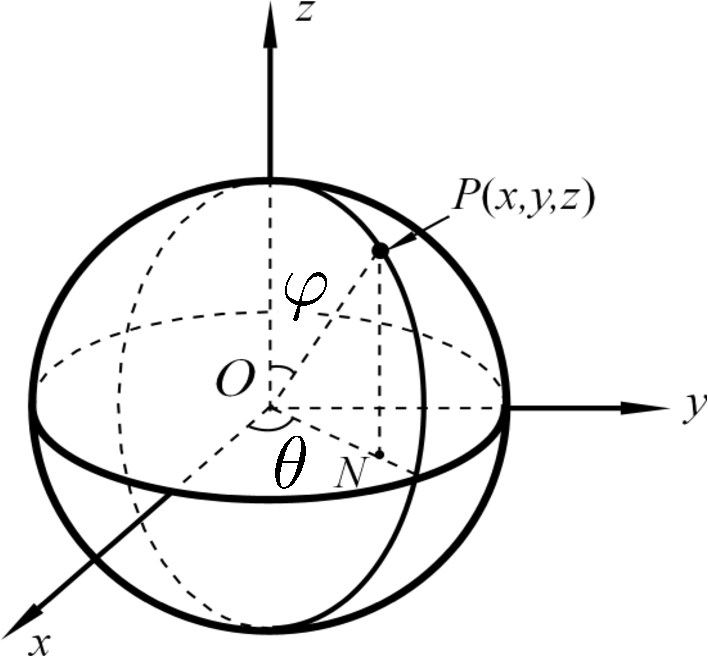
\includegraphics{./images/ch8/sphere.pdf}}
\end{center}

\subsection{一些特殊的曲面}

\subsubsection{【(坐标面内的曲线以坐标轴为旋转轴旋转所得的)旋转曲面】}

{\bf 定义:}曲线绕某条直线(轴)旋转一周所得的曲面。

{\bf 例:}求曲线$C:f(y,z)=0$绕$z$轴旋转一周所得曲面

$${f(\pm\sqrt{x^2+y^2},z)=0}$$

常见的旋转曲面包括:{\bf 旋转椭球面、旋转双曲面、旋转抛物面、圆锥面、圆柱面、\ldots}

{\bf 思考:}如果给定曲线不在某个坐标面内,绕某个坐标轴旋转,所得旋转曲面的方程如何求?

{\bf 例:}已知两点$A(1,0,0)$和$B(0,1,1)$,求直线$AB$绕$z$轴旋转一周所得曲面的方程。

$$AB:\;\df{x-1}{-1}=\df y1=\df z1,$$

$$x^2+y^2=2(z-\df12)^2+1$$

{\bf 思考:}空间一条直线绕另一条直线旋转,可能得到怎样的曲面?

{\bf 例:}求直线$l:\df{x}{a}=\df{y-b}0=z$绕$z$轴旋转一周所得曲面方程,并指出该曲面
的类型。

{\bf 思考:}如果旋转轴不是坐标轴,曲面的方程该如何表示?

\subsubsection{【柱面】}

由平行于定直线并沿某曲线移动的直线描绘出的轨迹称为{\bf 柱面},
定曲线称为其{\bf 准线},动直线称为其{\bf 母线}

{\bf 例:}曲线$C:F(x,y)=0$沿$z$轴方向运动的轨迹

$${S:\{(x,y,z)\in\mathbb{R}^3|F(x,y)=0\}}$$

\begin{center}
	\resizebox{!}{4cm}{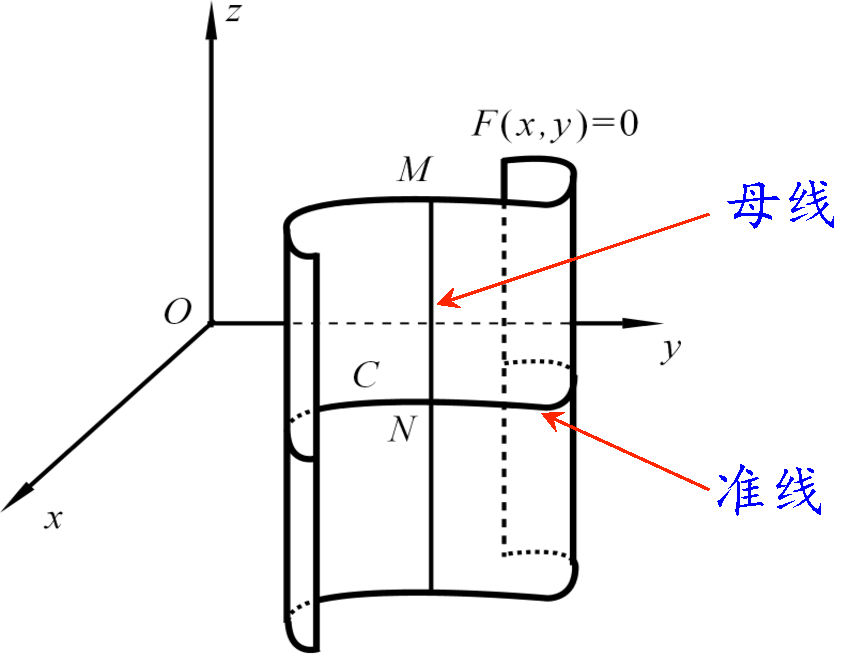
\includegraphics{./images/ch8/cyCurve.pdf}}
	
	P46-图8.3.14
\end{center}

\begin{center}
	\resizebox{!}{5cm}{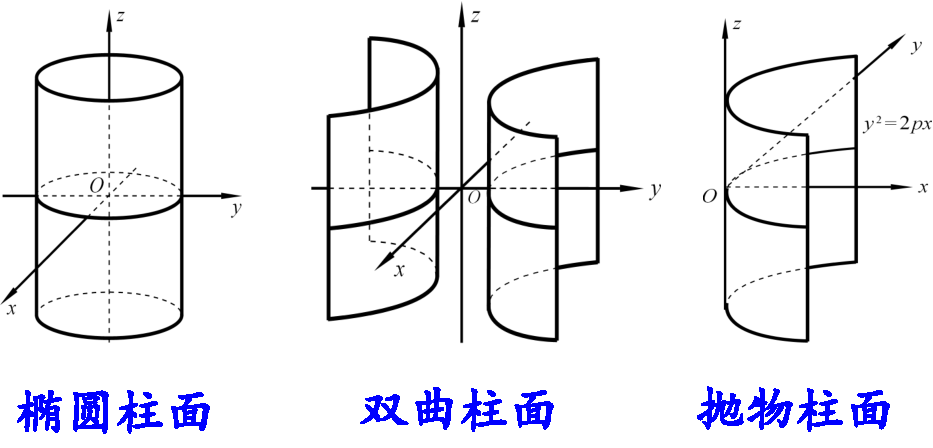
\includegraphics{./images/ch8/cylins.pdf}}
	
	P47-图8.3.15
\end{center}

{\bf 思考:}垂直于某个坐标面的柱面,其方程有何特点?

{\bf 例:}垂直于$xOy$平面,则方程中不包含$z$!

{\bf 思考:}如果移动的轨迹不是某个坐标轴,曲面的方程该如何表示?

{\bf 注:}参见辅导书(上)-P272!

\subsection{二次曲面}

{\bf 定义:}三元二次多项式方程所对应的空间曲面

\begin{eqnarray*}
	a_1x^2+a_2y^2+a_3z^2+b_1xy+b_2yx+b_3zx& &\\
	+c_1x+c_2y+c_3z+d & = & 0\\
	(a_1^2+a_2^2+a_3^2\ne 0)& &
\end{eqnarray*}

常见的二次曲面:

\subsubsection{【椭球面】}

$${\df{x^2}{a^2}+\df{y^2}{b^2}+\df{z^2}{c^2}=1}$$

\begin{center}
	\resizebox{!}{3.5cm}{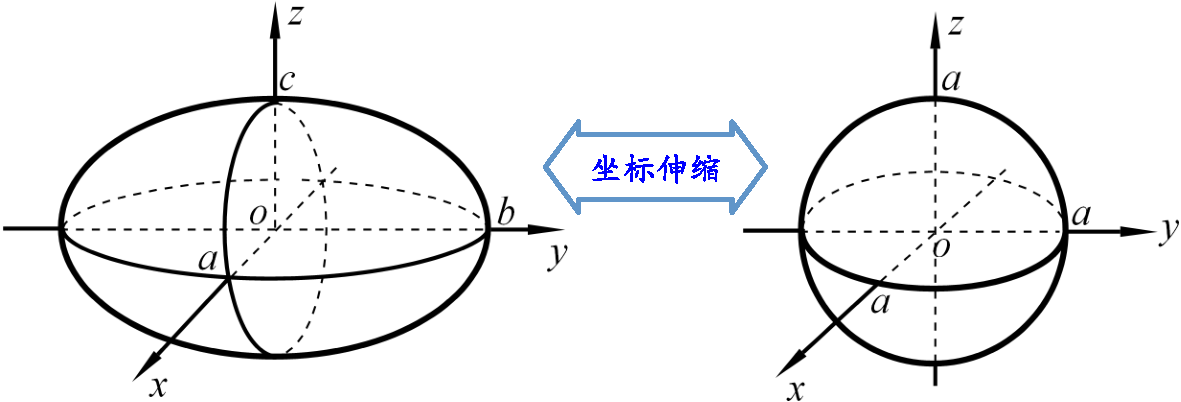
\includegraphics{./images/ch8/quaEllipse.pdf}}
\end{center}

参数方程:

$${x=a\sin\varphi\cos\theta,\;y=b\sin\varphi\sin\theta,\;z=c\cos\varphi},
{(0\leq\theta\leq
2\pi,0\leq\varphi\leq\pi)}$$

\subsubsection{【单叶双曲面】}

$${\df{x^2}{a^2}+\df{y^2}{b^2}-\df{z^2}{c^2}=1}$$

参数方程:

$$x=a\sec\varphi\cos\theta,\;y=b\sec\varphi\sin\theta,\;z=c\tan\varphi,
(0\leq\theta\leq 2\pi,0\leq\varphi\leq\pi)$$

\subsubsection{【双叶双曲面】}

$${-\df{x^2}{a^2}-\df{y^2}{b^2}+\df{z^2}{c^2}=1}$$

参数方程:

$$\left\{\begin{array}{l}
	x=a\tan\varphi\cos\theta,\\
	y=b\tan\varphi\sin\theta,\\
	z=c\sec\varphi.
\end{array}\right.(0\leq\theta\leq 2\pi,0\leq\varphi\leq\pi)$$

\subsubsection{【椭圆抛物面】}

$${z=\df{x^2}{a^2}+\df{y^2}{b^2}}$$

参数方程:

$$\left\{\begin{array}{l}
	x=au\cos\theta,\\
	y=bu\sin\theta,\\
	z=u^2.
\end{array}\right.(0\leq\theta\leq 2\pi,u\geq 0)$$

\subsubsection{【双曲抛物面(马鞍面)】}

$${z=\df{x^2}{a^2}-\df{y^2}{b^2}}$$

$$x=au\sec\theta,\;y=bu\tan\theta,\;z=u^2,
(0\leq\theta\leq 2\pi,u\geq
0)$$

{\bf 例:}证明:$z=xy$对应的曲面为双曲抛物面

\begin{center}
	\resizebox{!}{4cm}{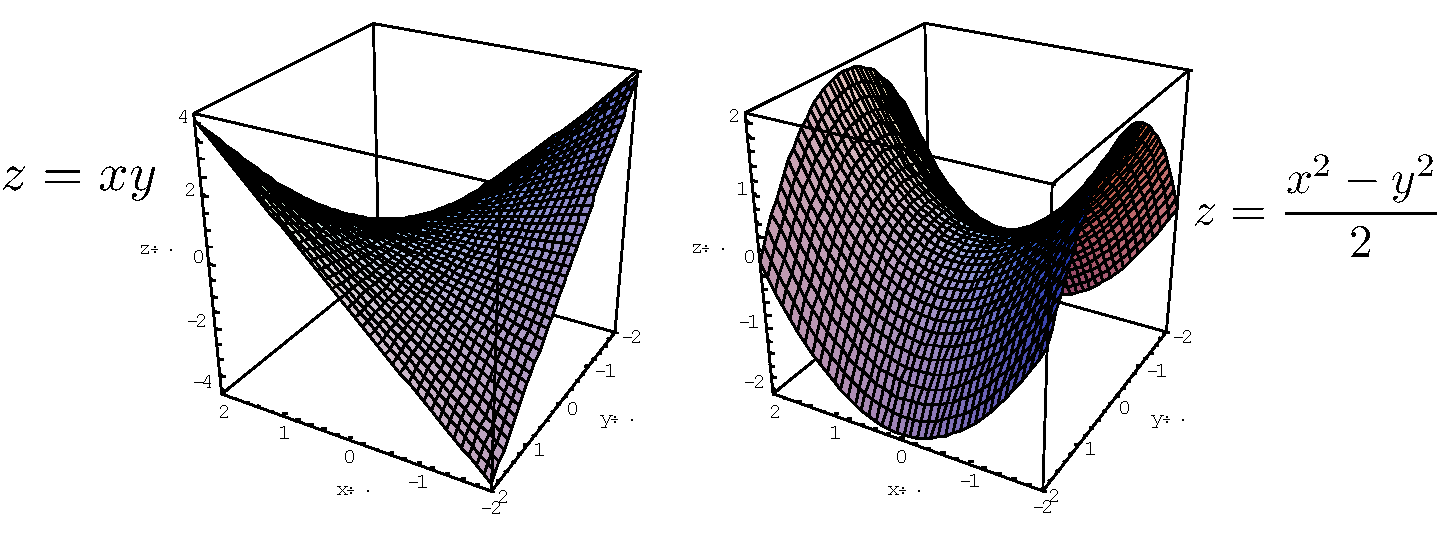
\includegraphics{./images/ch8/diffArch.pdf}}
\end{center}

{\bf (二维)坐标旋转公式:}{ (逆时针旋转$\theta$)}
$${\left\{\begin{array}{l}
	X=x\cos\theta+y\sin\theta\\
	Y=-x\sin\theta+y\cos\theta
\end{array}\right.}$$

\subsubsection{【椭圆锥面】}

$${\df{x^2}{a^2}+\df{y^2}{b^2}-\df{z^2}{c^2}=0}$$

参数方程:

$$\left\{\begin{array}{l}
	x=au\cos\theta,\\
	y=bu\sin\theta,\\
	z=u.
\end{array}\right.(0\leq\theta\leq 2\pi,u\in\mathbb{R})$$

\subsection{直纹面}

{\bf 问题:}空间直线按照一定的规律运动会产生什么样的曲面?

\begin{center}
	\resizebox{!}{5cm}{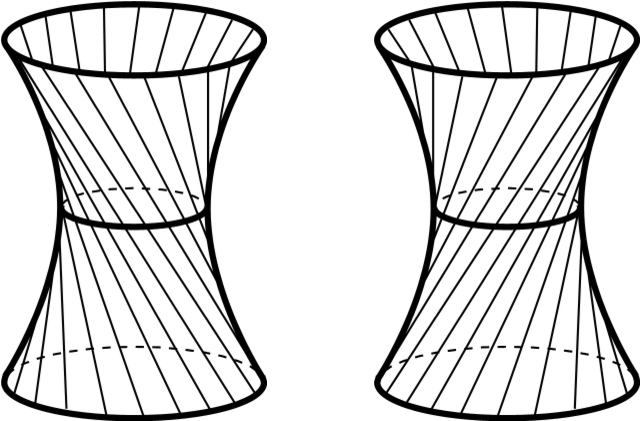
\includegraphics{./images/ch8/rtLHypo.pdf}}
	
	单叶双曲面:$\df{x^2}{a^2}+\df{y^2}{b^2}-\df{z^2}{c^2}=1$
\end{center}

{\bf 习题8.3-10:}证明:单叶双曲面$\df{x^2}{a^2}+\df{y^2}{b^2}-\df{z^2}{c^2}=1$
是由两组直线
$$\left\{\begin{array}{l}
	u\left(\df xa+\df zc\right)+v\left(1\pm\df yb\right)=0\\[1em]
	u\left(1\mp\df yb\right)+v\left(\df xa-\df zc\right)=0
\end{array}\right.\quad (u^2+v^2\ne 0)$$
生成的直纹面。即:对于单叶双曲面上的任意点,两组直线中各有一条通过改点。

{\bf 例:}判断以下曲面的类型及其特征
\begin{enumerate}[(1)]
  \setlength{\itemindent}{1cm}
  \item $x^2+y^2+z^2+2x-2y=0$
  \item $x^2-y^2+z^2+2x-2y=0$
  \item $x^2+y^2+z^2+2x-2y=2$
  \item $x^2-y^2+z^2+2x-2y=2$
  \item $x^2-y^2+z^2+2x-2y=-2$
  \item $x^2+y^2+z^2+2x+2y=2$
  \item $x^2+y^2-z^2+2xy=0$
  \item $x^2+y^2-z=0$
  \item $x^2-y^2-z=0$
  \item $x^2-z=0$
  \item $x^2-y+z=0$
\end{enumerate}

\section{空间曲线}

\subsection{空间曲线的参数方程}

{\bf Insight:}任意曲线都可以视为动点的运动轨迹

$${x=x(t),\;y=y(t),\;z=z(t)}$$

{\bf 例:}以下方程表示何种曲线
\begin{enumerate}
  \item $x=\cos t,\;y=\sin t,\;z=t\;(t\in\mathbb{R})$ 
  \item $x=t\cos t,\;y=t\sin t,\;z=t\;(t\in\mathbb{R})$ 
\end{enumerate}

\subsection{空间曲线的一般式方程}

{\bf Insight:}空间曲线可视为两个(或更多)曲面的交线

$${\left\{\begin{array}{l}
	F(x,y,z)=0,\\ G(x,y,z)=0
\end{array}\right.}$$

{\bf P59-例3:}以下方程对应何种曲线

$$\left\{\begin{array}{l}
	z=\sqrt{R^2-x^2-y^2},\\ x^2+y^2-Rx=0
\end{array}\right. \quad{\mbox{(Viviani曲线)}}$$

\begin{center}
	\resizebox{!}{4.5cm}{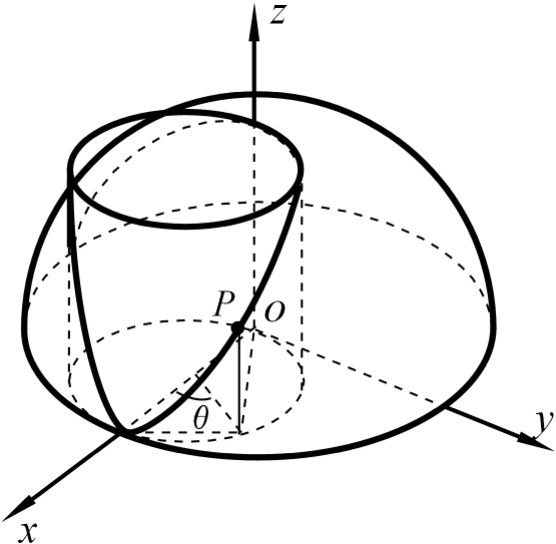
\includegraphics{./images/ch8/viviani.pdf}}
\end{center}

\subsection{空间曲线的投影}

{\bf P60-例5:}求空间曲线$C:\left\{\begin{array}{l}
	x^2+y^2+z^2=1\\ x^2+(y-1)^2+(z-1)^2=1
\end{array}\right.$
在$xOy$平面上的投影曲线方程。

\begin{center}
	\resizebox{!}{3.5cm}{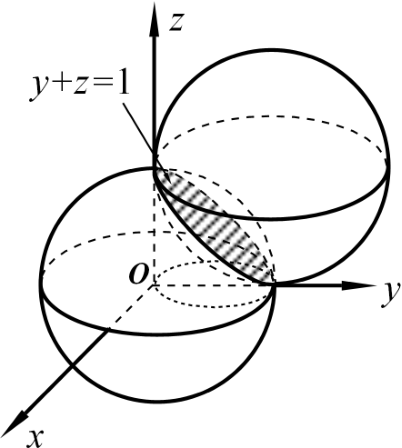
\includegraphics{./images/ch8/shaBall.pdf}}
\end{center}

{\bf Insight:}曲线在$xOy$上的投影:变量$x,y$满足的柱面方程与$xOy$平面的交线

空间曲线:
$$C:\left\{\begin{array}{l}
	F(x,y,z)=0\\ G(x,y,z)=0
\end{array}\right.$$
消去$z$,所得方程
$$H(x,y)=0$$

{\bf 注:}$H(x,y)=0$既可以表示$xOy$平面内的一条曲线({\bf $C$的投影曲线}),
也可以表示曲线$C$关于$xOy$平面的({\bf 投影柱面})

\subsection{参数方程与投影曲线}

{曲线$C$:}
$$x=x(t),\;y=y(t),\;z=z(t)\;(t\in[t_0,t_1])$$ 
{曲线$C$在$xOy$平面内的投影曲线:}
$$x=x(t),\;y=y(t),\;{z=0}\;(t\in[t_0,t_1])$$ 

{\bf 思考:}如果直接在曲线的一般式方程中令$z=0$,所得是否即为其在$xOy$平面内的投影曲线?
(${\times}$)

{\bf P59-例4:}圆柱螺旋线在三个坐标面上的投影分别是什么曲线?

\begin{center}
	\resizebox{!}{5cm}{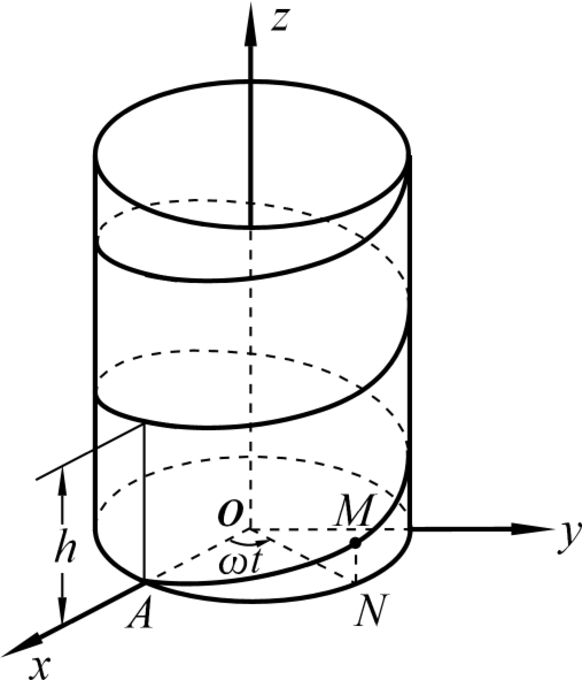
\includegraphics{./images/ch8/cylinderCurve.pdf}}
\end{center}

$$x=R\sin t, y=R\cos t, z=at,(t\in\mathbb{R})$$

{\bf P61-例6:}求Viviani曲线在各坐标面上的投影曲线,并由此写出Viviani曲线的参数方程。

\begin{center}
	\resizebox{!}{6.5cm}{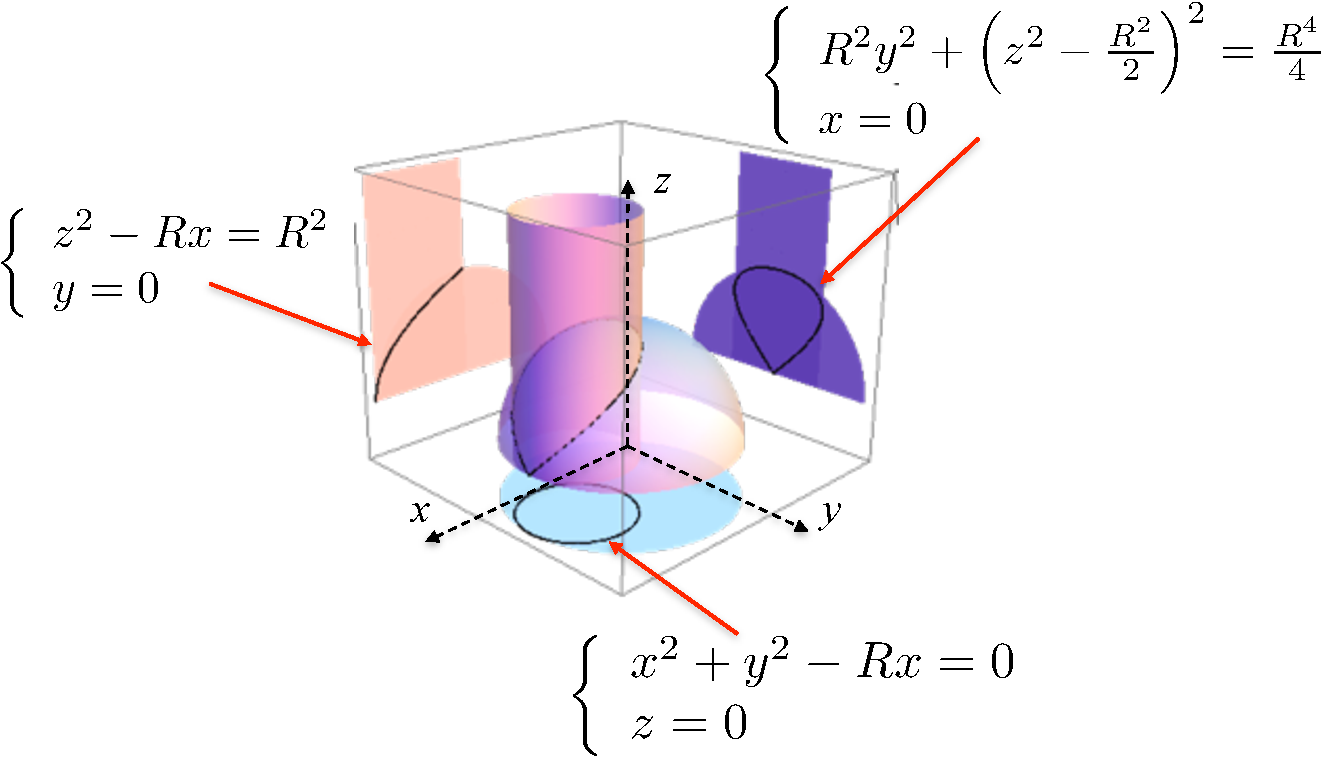
\includegraphics{./images/ch8/vivianiPara.pdf}}
\end{center}

$${x=\df R2(1+\cos\theta),\;y=\df
R2\sin\theta,\;z=R\sin\df{\theta}{2},\;\theta\in[0,2\pi]}$$

{\bf 辅导书(上)-P284-例5-24:}证明曲线$$C:\left\{\begin{array}{l}
	4x-5y-10z-20=0,\\ \df{x^2}{25}+\df{y^2}{16}-\df{z^2}4=1
\end{array}\right.$$
为两条相交的直线,求其方程。

[提示]:联立化简,得$x=5,y=-4$,两直线方程
$$\df{x-5}0=\df{y}{-2}=\df z1,\quad \df x5=\df{y+4}0=\df z2$$
交点$(5,-4,2)$

{\bf 辅导书(上)-P284-例5-25:}将曲线方程$$C:\left\{\begin{array}{l}
	2y^2+z^2+4x=z\\ y^2+3z^2-8x=12x
\end{array}\right.$$
换成母线分别平行于$x$轴和$y$轴的柱面的交线的形式。

$$5y^2+4z^2=14z,\;5z^2-20x=23z$$
\subsection{曲面的截痕曲线}

{\bf 截痕曲线:}特定平面与曲面的交线

{\bf 例:}试用考查以下曲面的截痕曲线:
\begin{enumerate}[(1)]
  \setlength{\itemindent}{1cm}
  \item 单叶双曲面
  \item 双叶双曲面
  \item 双曲抛物面
\end{enumerate}

\section{习题课}

\subsection{本章小结}

\begin{enumerate}
  \item 向量及其表示:长度+方向
  \item 向量运算
  \begin{itemize}
    \item 线性运算:平移、伸缩
    \item 点乘:投影
    \item 叉乘:右手法则、平行四边形面积
    \item 混合积:体积
  \end{itemize}
  \item 空间对象的向量表示
  \begin{enumerate}
	\item 如何根据空间对象的特征给出其方程? 
	\item 如何由空间对象的方程发现其特征? 
  \end{enumerate}
  \begin{itemize}
	\item 位置$\to$向径 
	\item 距离$\to$模 
	\item 平行/垂直$\to$内/外积 
	\item 夹角$\to$内积 
	\item 投影$\to$内积 
	\item 自由度/维度 
    \begin{itemize}
      \item 平面$\to$2维$\to$1个方程
      \item 直线$\to$1维$\to$2个方程
    \end{itemize}
    \item 方程的次数
    \begin{itemize}
      \item 平面/直线$\to$1次方程
    \end{itemize}
  \end{itemize}
\end{enumerate}

\subsection{综合练习}

\subsubsection{【向量及其运算】}

{\bf 例:}已知一向量的模为$2$,且与$x$轴和$y$轴的夹角相同,与$z$轴的夹角是
它们的两倍,求此向量。

{\bf 例:}设$\bm{a},\bm{b}$均为非零向量,且$|\bm{b}|=1$,二者夹角为$\pi/3$,求
$$\limx{0}\df{|\bm{a}+x\bm{b}|-|\bm{a}|}{x}$$

{\bf 辅导书(上)-P285-例5:}已知$\bm{a}+3\bm{b}$与$7\bm{a}-5\bm{b}$垂直,
$\bm{a}-4\bm{b}$与$7\bm{a}-2\bm{b}$垂直,求$\bm{a}$和$\bm{b}$的夹角

[提示]:
$$7|\bm{a}|^2+16\bm{a}\cdot\bm{b}-15|\bm{b}|^2=0,\;
7|\bm{a}|^2-30\bm{a}\cdot\bm{b}+8|\bm{b}|^2=0$$
解得$|\bm{a}|=|\bm{b}|$,$\bm{a}\cdot\bm{b}=\df12|\bm{b}|^2$,从而
夹角$\df{\pi}3$

{\bf 例:}已知平行四边形的两对角线向量分别为$\bm{A}=\bm{m}+2\bm{n}$,
$\bm{B}=2\bm{m}-4\bm{n}$,其中$|\bm{m}|=1,|\bm{n}|=2$,
$\bm{m}$和$\bm{n}$的夹角为$\pi/6$,求该平行四边形的面积。

{\bf 例:}试用向量方法证明正弦定理
$$\df{a}{\sin A}=\df{b}{\sin B}=\df{c}{\sin C}$$

\subsubsection{【平面与直线】}

{\bf 1. 平面束}

{\bf 例:}证明:$$\lambda(A_1x+B_1y+C_1z+D_1)+\mu(A_2x+B_2y+C_2z+D_2)=0$$
(其中$\lambda,\mu$不全为零)为过直线
$$L:\left\{\begin{array}{l}
	A_1x+B_1y+C_1z+D_1=0\\
	A_2x+B_2y+C_2z+D_2=0
\end{array}\right.$$
的{\bf 平面束}。

前例可用平面束求解,首先求直线的一般式方程:
$$\left\{\begin{array}{l}x-5y-4=0\\ y-2z+3=0\end{array}\right.$$
然后给出平面束方程,带入$M$的坐标确定$\lambda=8,\mu=-9$

{\bf 辅导书(上)-P277-5-11:}过点$M(3,1,-2)$和直线$\df{x-4}5=\df{y+3}2=\df z1$
的平面

[提示]:直线上任取一点$M_1(4,-3,0)$,求得法向量
$$\bm{n}=\bm{s}\times\bm{MM_1}=(-8,9,22)$$
所求平面
$$8x-9y-22x-59=0$$

{\bf 例:}求过$z$轴,且与$yOz$的夹角为$\df{\pi}4$的平面方程。

{\bf 例:}求过直线
$$\left\{\begin{array}{l}
	x+5y+z=0\\
	x-z+4=0
\end{array}\right.$$
且与平面$\pi:x-4y-8z+12=0$的夹角为$\pi/4$的平面方程。

{\bf 2. 异面直线}

{\bf 辅导书(上)-P280-5-16:}已知直线
$$L_1:\left\{\begin{array}{l}
	x+y+z+1=0\\
	2x-y+3z+4=0
\end{array}\right.
\quad
L_2:\left\{\begin{array}{l}
	x=-1+2t\\
	y=-t\quad(t\in\mathbb{R})\\
	z=2-2t
\end{array}\right.
$$
\begin{enumerate}[(1)]
  \setlength{\itemindent}{1cm}
  \item 证明两直线异面;
  \item 求两直线间的距离;
  \item 求二者的公垂线方程。
\end{enumerate}

[提示]:$L_1,L_2$的标准式方程
$$\df{x+3}4=\df{y-1}{-1}=\df{z-1}{-3},\quad
\df{x+1}2=\df y{-1}=\df{z-2}{-2}$$
(1)任取两点与方向向量做混合积,非零,故不共面。

(2)法一:两直线各取一点,对应在$\bm{s_1}\times\bm{s_2}=(-1,2,-2)$上的投影。

$$d=2$$

法二:将(1)中的混合积(平行六面体面积)除以$|\bm{s_1}\times\bm{s_2}|$(底面积)

(3)法一:分别求过两条直线与公垂线方向平行的平面,联立即可。

$$\left\{\begin{array}{l}
	8x+11y+7z+6=0\\
	2x+2y+z=0
\end{array}\right.$$

法二:设出公垂线与两条直线的交点,利用公垂线的参数方程和直线的参数方程求出参数值即可。

$$\df{x-1}{-1}=\df y2=\df{z+2}{-2}$$

\subsubsection{【曲面与曲线】}

{\bf 辅导书(上)-P290-例18:}由椭球面$\df{x^2}{a^2}+\df{y^2}{b^2}+\df{z^2}{c^2}=1$的
中心引三条相互垂直的射线,分别交椭球面于三点$P_i(i=1,2,3)$,
记$|\bm{OP}_i|=r_i(i=1,2,3)$,证明:
$$\df{1}{r_1^2}+\df{1}{r_2^2}+\df{1}{r_3^2}
=\df{1}{a^2}+\df{1}{b^2}+\df{1}{c^2}$$

{\bf 旋转体}

{\bf 习题8.3-8:}证明:到定直线及该直线上一定点的距离平方和为常数的动点轨迹为一个旋转曲面。

{\bf 习题8.4-10:}证明:空间曲线$\Gamma:x=\varphi(t),y=\phi(t),z=\psi(t)$绕$z$轴旋转一周所得
旋转曲面的参数方程为:
$$\left\{\begin{array}{l}
	x=\sqrt{\varphi^2(t)+\phi^2(t)}\cos\theta,\\
	y=\sqrt{\varphi^2(t)+\phi^2(t)}\sin\theta,\\
	z=\psi(t)
\end{array}\right.$$

{\bf 辅导书(上)-P282-例5-21:}求直线$l:\df{x}{a}=\df{y-b}0=z$绕$z$轴旋转一周所得曲面方程,并指出该曲面
的类型。

$$\left\{\begin{array}{l}
x=\sqrt{a^2t^2+b^2}\cos\theta,\\ y=\sqrt{a^2t^2+b^2}\sin\theta,\\ z=t
\end{array}\right.$$
也即
$$x^2+y^2=a^2z^2+b^2$$
\begin{enumerate}[(1)]
  \setlength{\itemindent}{1cm}
  \item $a=b=0$,$z$轴
  \item $a\ne0,b=0$,圆锥面
  \item $a\ne0,b\ne0$,单叶双曲面
  \item $a=0,b\ne0$,圆柱面
\end{enumerate}

{\bf 习题8.3-9:}已知点$A(1,0,0)$与点$B(0,1,1)$,直线$AB$绕$z$轴旋转一周
所成的旋转曲面为$S$,求$S$与$z=0$、$z=1$所围成的立体体积。



{\bf 例:}求空间曲线$$\left\{\begin{array}{l}
F(x,y,z)=0\\ G(x,y,z)=0
\end{array}\right.$$绕直线
$$\df{x-a}m=\df{y-b}n=\df{z-c}p$$
旋转一周所得曲面的方程。

{\bf 柱体:}

{\bf 例:}设柱面的母线平行于直线$x=y=z$,准线为$x+y-z=1,x-y+z=0$,求柱面的方程。

{\bf 例:}求通过曲线$\left\{\begin{array}{l}
	x^2+y^2+z^2=8\\
	x^2+z^2-y^2=0
\end{array}\right.$,且母线分别平行于$x$轴,$y$轴和$x=y=z$的柱面方程。

{\bf  辅导书(上)-P282-例5-22:}求母线平行于$x=y=z$,准线为
$\left\{\begin{array}{l}
	x^2+y^2+z^2=1\\ x+y+z=0
\end{array}\right.$的柱面方程

[提示]:任取准线上一点$(u,v,w)$,过其的母线为
$$x-u=y-v=z-w,$$
将其与准线方程联立,消除$u,v,w$得
$$x^2+y^2+z^2-xy-yz-zx=\df32$$

{\bf 注:}关于各种柱面的求法,可参见辅导书(上)-P272

{\bf 例:}求空间曲线$\Gamma:\left\{\begin{array}{l}
F(x,y,z)=0\\ G(x,y,z)=0
\end{array}\right.$在平面$\pi:Ax+By+Cz+D=0$上的投影曲线方程。

[提示]:任取$(u,v,w)\in\Gamma$,其到$\pi$的垂线
$$\df{x-u}A=\df{y-v}B=\df{z-w}C,$$
将其与曲面方程联立,消去$u,v,w$,即得$\Gamma$沿$\pi$的法向运动所得柱面。联系该柱面与
平面方程,即为所求。

{\bf 思考:}若$\Gamma$表示为参数方程,如何求其沿$(m,n,p)$的投影柱面?

$$x=x(t)+mu,y=y(t)+nu,\;z=z(t)+pu,\;(t,u\in\mathbb{R})$$

\newpage

\section*{课后作业}
\addcontentsline{toc}{section}{课后作业}

{\bf 【必作题】}

\begin{itemize}
  \setlength{\itemindent}{1cm}
  \item 习题8.1:4,9,11,12,14(1),16,19,24
  \item 习题8.2:11,14,15,16,17,19,21
  \item 习题8.3:6,8,9
  \item 习题8.4:4,8,9,10,11
\end{itemize}

\bigskip

\hrule

\bigskip
\bigskip

{\bf 【思考题】}

% \begin{itemize}
%   \setlength{\itemindent}{1cm}
%   \item 习题8.1:21
%   \item 习题8.2:20,24
% \end{itemize}

1、设$\bm{a},\bm{b}$均为非零向量,且$|\bm{b}|=1$,二者夹角为$\pi/3$,求
$$\limx{0}\df{|\bm{a}+x\bm{b}|-|\bm{a}|}{x}$$

2、已知$\bm{a},\bm{b}$均为非零向量,向量$\bm{a}+3\bm{b}$与$7\bm{a}-5\bm{b}$垂直,
$\bm{a}-4\bm{b}$与$7\bm{a}-2\bm{b}$垂直,求$\bm{a}$和$\bm{b}$的夹角。

3、求过直线
$$\left\{\begin{array}{l}
	x+y=0\\
	x-y=0
\end{array}\right.$$
且与平面$\pi:x-4y-8z+12=0$的夹角为$\pi/4$的平面方程。

4、叙述如何求空间曲线$$\left\{\begin{array}{l}
F(x,y,z)=0\\ G(x,y,z)=0
\end{array}\right.$$绕直线
$$\df{x-a}m=\df{y-b}n=\df{z-c}p$$
旋转一周所得曲面的方程。(要求:写出思路和大致的解题步骤)

5、设柱面的母线平行于直线$x=y=z$,准线为$x+y-z=1,x-y+z=0$,求柱面的方程。

6、求母线平行于$x=y=z$,准线为
$\left\{\begin{array}{l}
	x^2+y^2+z^2=1\\ x+y+z=0
\end{array}\right.$的柱面方程。

7、已知直线
$$L_1:\left\{\begin{array}{l}
	x+y+z+1=0\\
	2x-y+3z+4=0
\end{array}\right.
\quad
L_2:\left\{\begin{array}{l}
	x=-1+2t\\
	y=-t\quad(t\in\mathbb{R})\\
	z=2-2t
\end{array}\right.
$$
\begin{enumerate}[(1)]
  \setlength{\itemindent}{1cm}
  \item 证明两直线异面;
  \item 求两直线间的距离;
  \item 求二者的公垂线方程。
\end{enumerate}

\ifvisible

\newpage

\section*{第八章习题课课后作业(上交题)}

{\it (注:本次作业请务必抄题!)}

\bigskip

1、设$\bm{a},\bm{b}$均为非零向量,且$|\bm{b}|=1$,二者夹角为$\pi/3$,求
$$\limx{0}\df{|\bm{a}+x\bm{b}|-|\bm{a}|}{x}$$

2、已知$\bm{a},\bm{b}$均为非零向量,向量$\bm{a}+3\bm{b}$与$7\bm{a}-5\bm{b}$垂直,
$\bm{a}-4\bm{b}$与$7\bm{a}-2\bm{b}$垂直,求$\bm{a}$和$\bm{b}$的夹角。

3、求过直线
$$\left\{\begin{array}{l}
	x+y=0\\
	x-y=0
\end{array}\right.$$
且与平面$\pi:x-4y-8z+12=0$的夹角为$\pi/4$的平面方程。

4、叙述如何求空间曲线$$\left\{\begin{array}{l}
F(x,y,z)=0\\ G(x,y,z)=0
\end{array}\right.$$绕直线
$$\df{x-a}m=\df{y-b}n=\df{z-c}p$$
旋转一周所得曲面的方程。(要求:写出思路和大致的解题步骤)

5、设柱面的母线平行于直线$x=y=z$,准线为$x+y-z=1,x-y+z=0$,求柱面的方程。

6、求母线平行于$x=y=z$,准线为
$\left\{\begin{array}{l}
	x^2+y^2+z^2=1\\ x+y+z=0
\end{array}\right.$的柱面方程。

7、已知直线
$$L_1:\left\{\begin{array}{l}
	x+y+z+1=0\\
	2x-y+3z+4=0
\end{array}\right.
\quad
L_2:\left\{\begin{array}{l}
	x=-1+2t\\
	y=-t\quad(t\in\mathbb{R})\\
	z=2-2t
\end{array}\right.
$$
\begin{enumerate}[(1)]
  \setlength{\itemindent}{1cm}
  \item 证明两直线异面;
  \item 求两直线间的距离;
  \item 求二者的公垂线方程。
\end{enumerate}

\newpage

{\bf 关于不定积分的一个问题:}

\begin{eqnarray*}
	\dint\tan x\d x & = & \dint\tan x\sec x\cos x\d x=\dint\cos x\d\sec x\\
	& = & \cos x\sec x-\dint\sec x\d\cos x\\
	& = & 1+\dint\sec x\sin x\d x
	= 1+\dint\tan x\d x
\end{eqnarray*}

由此推出:$0=1$?

{\bf 解释:}不定积分表示的是(之间相差常数的)一类函数,所以等式两边消去时允许出现任意的值。
事实上,如果改为定积分,以上情况就不会出现了,例如在$[0,\pi/4]$上的定积分。

提示:如果计算不定积分时,出现了某个孤立的常数,可以将该常数直接“舍去”,或者理解为“吸收”
到不定积分之中。

\newpage

{\bf 关于习题8.1-24的不同解答:}

\begin{center}
	\resizebox{13cm}{!}{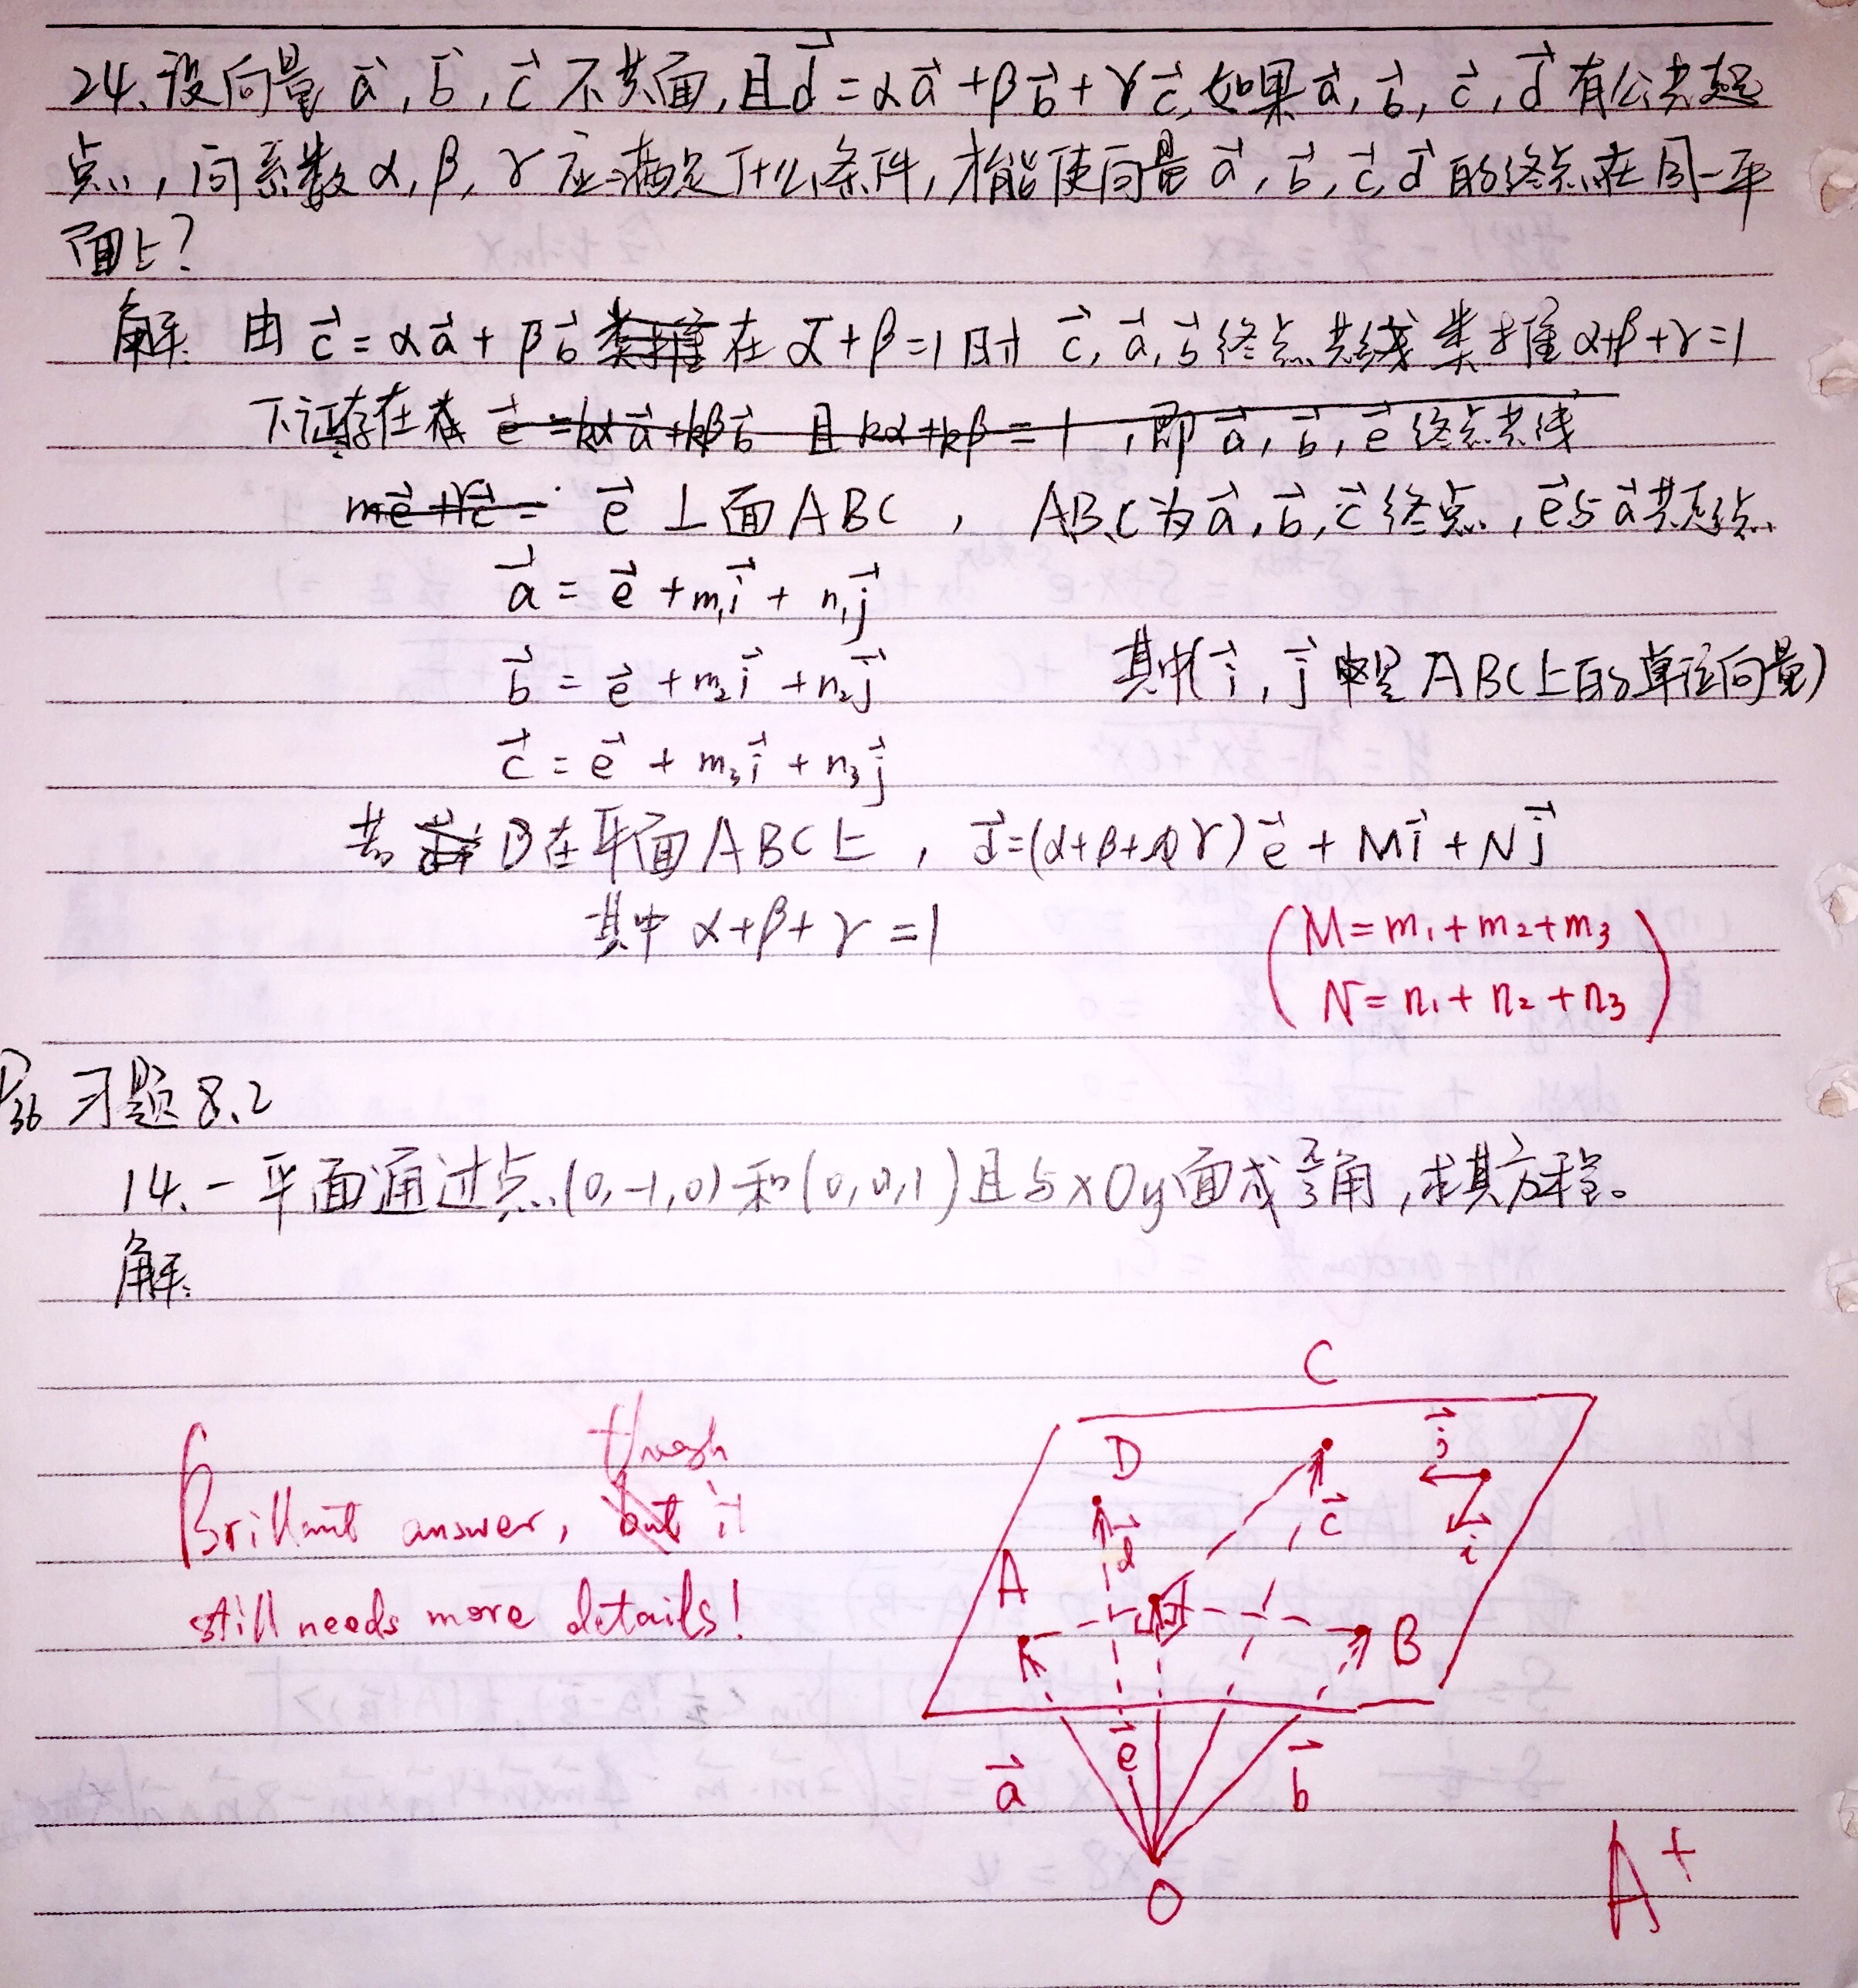
\includegraphics{./images/ch8/abcd-briAn.jpg}}
\end{center}

{\it 非常精妙,具有很好的几何想象和分析能力!}

\begin{center}
	\resizebox{13cm}{!}{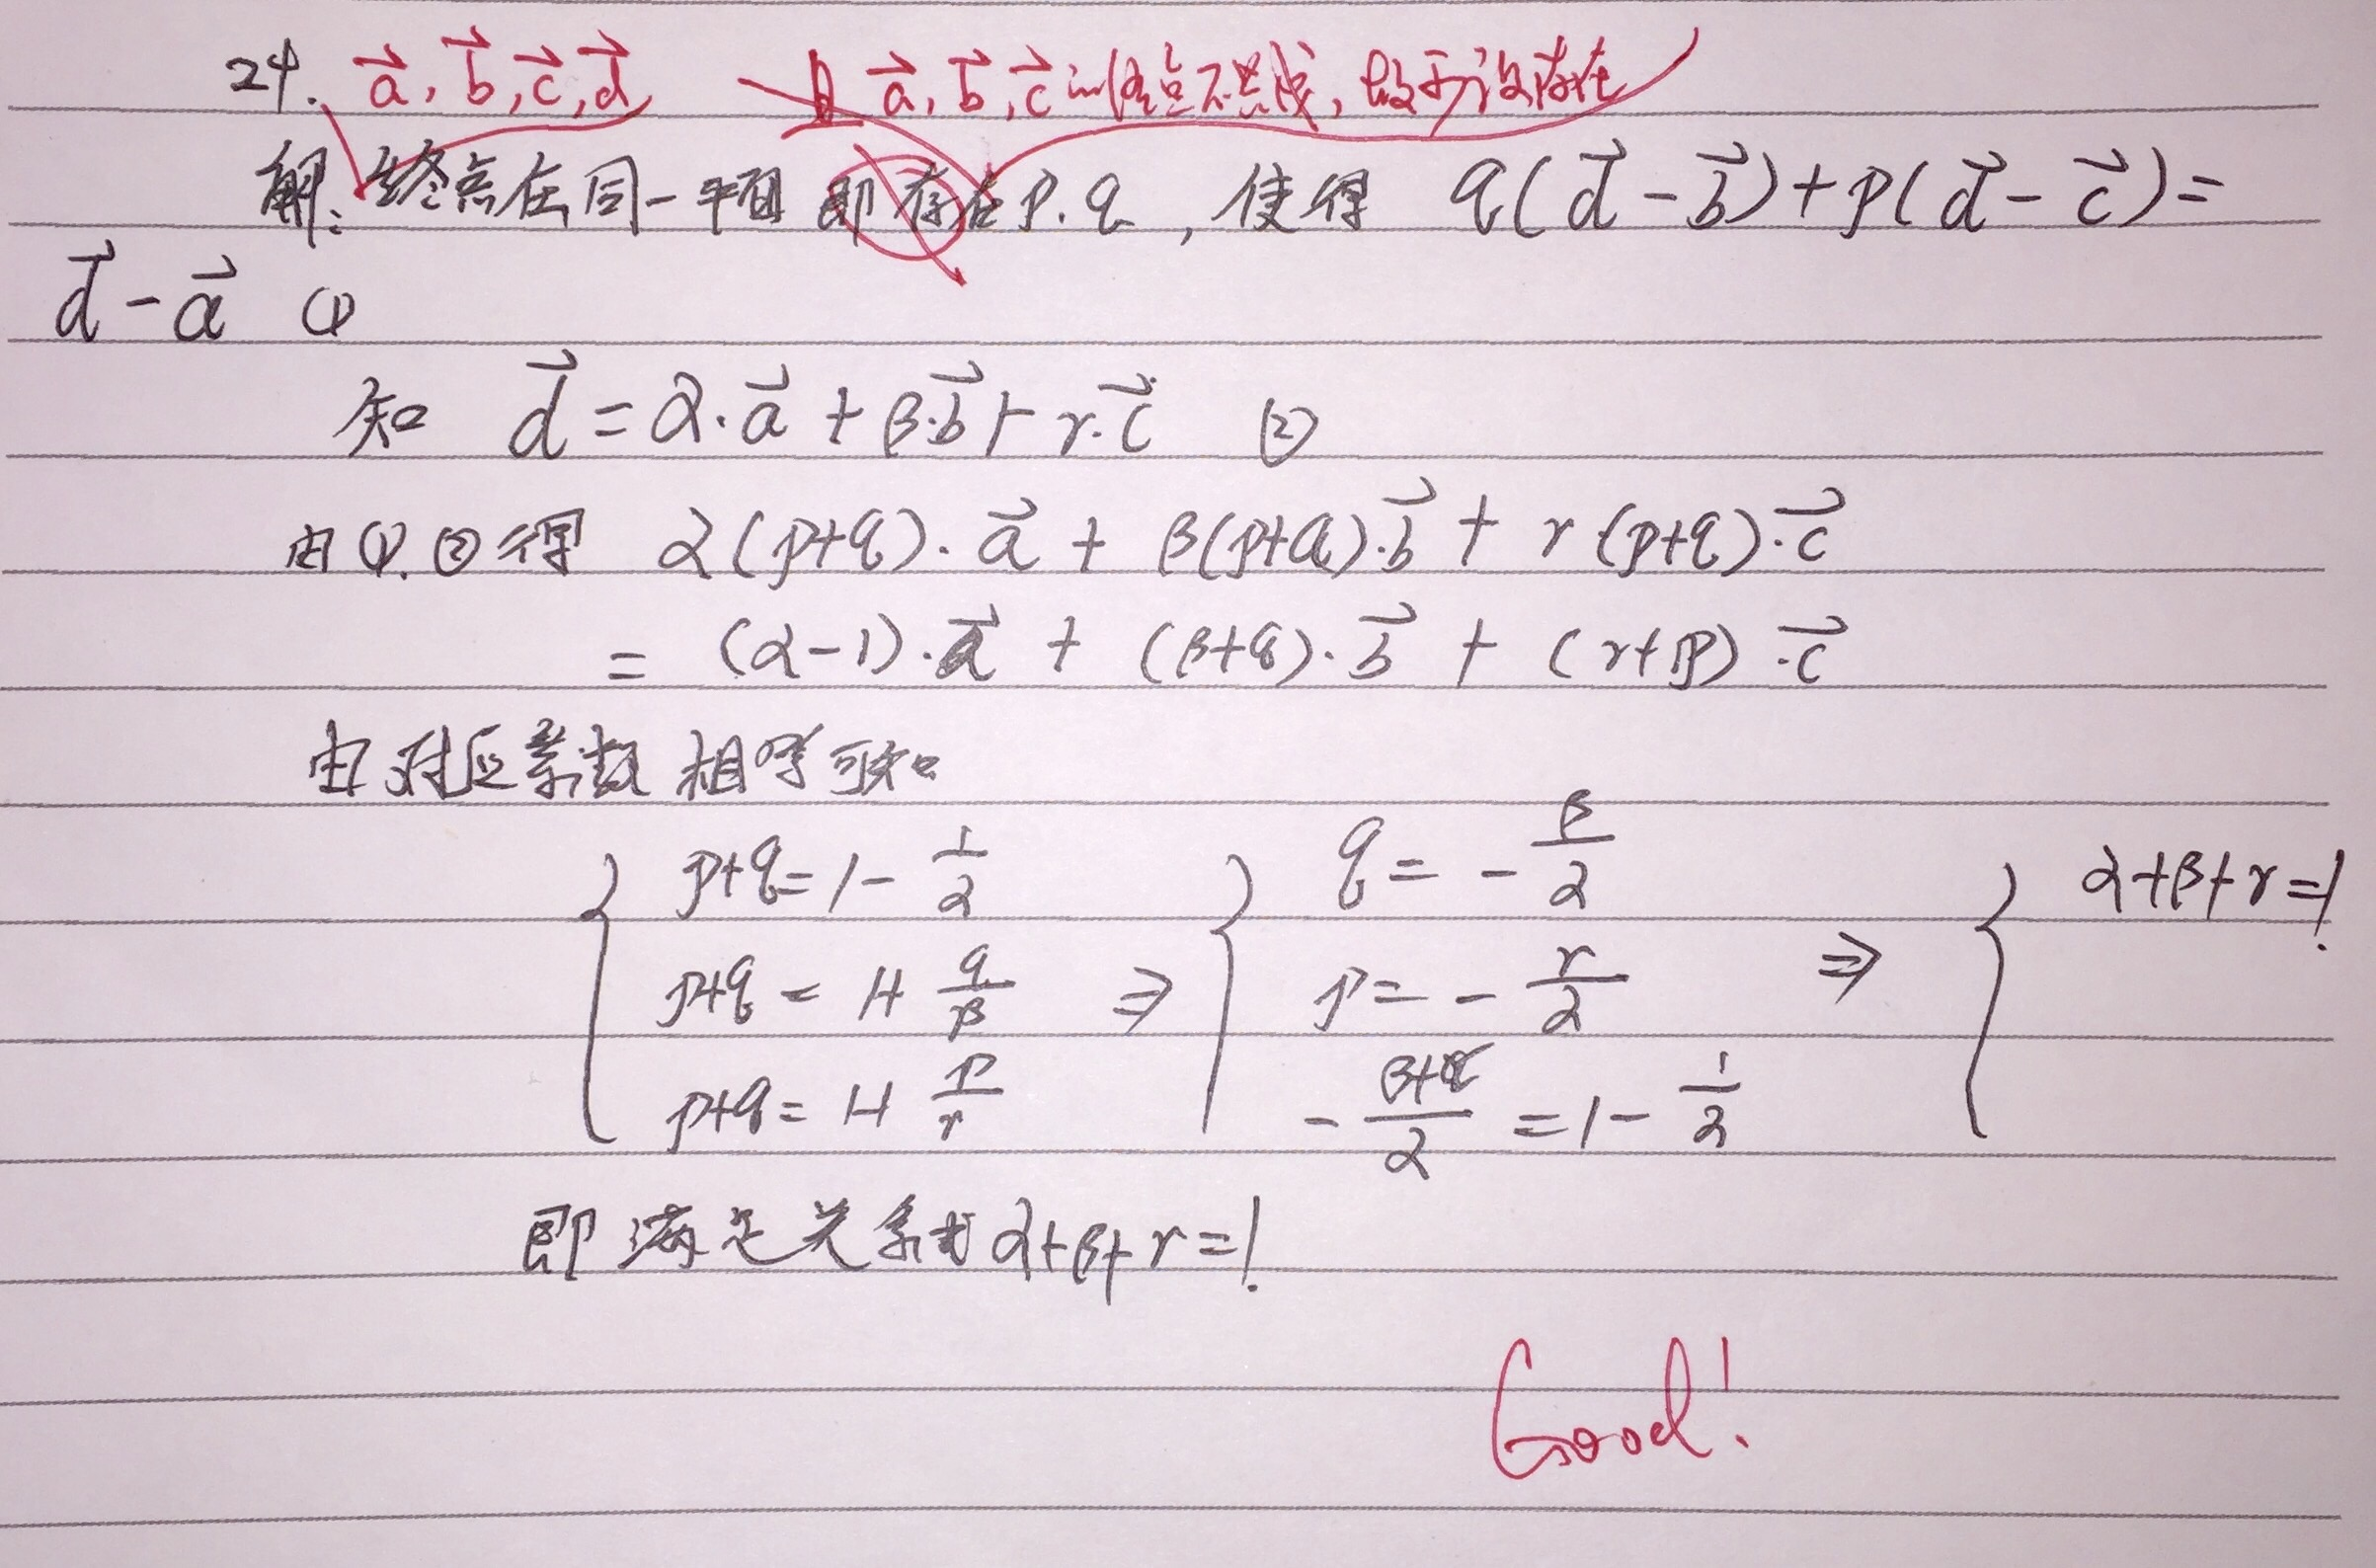
\includegraphics{./images/ch8/abcd-briAn-2.jpg}}
\end{center}

{\it 用纯代数方法求解,十分巧妙!}

\newpage

{\bf 第八章内容小结(手写版)}

\resizebox{!}{8cm}{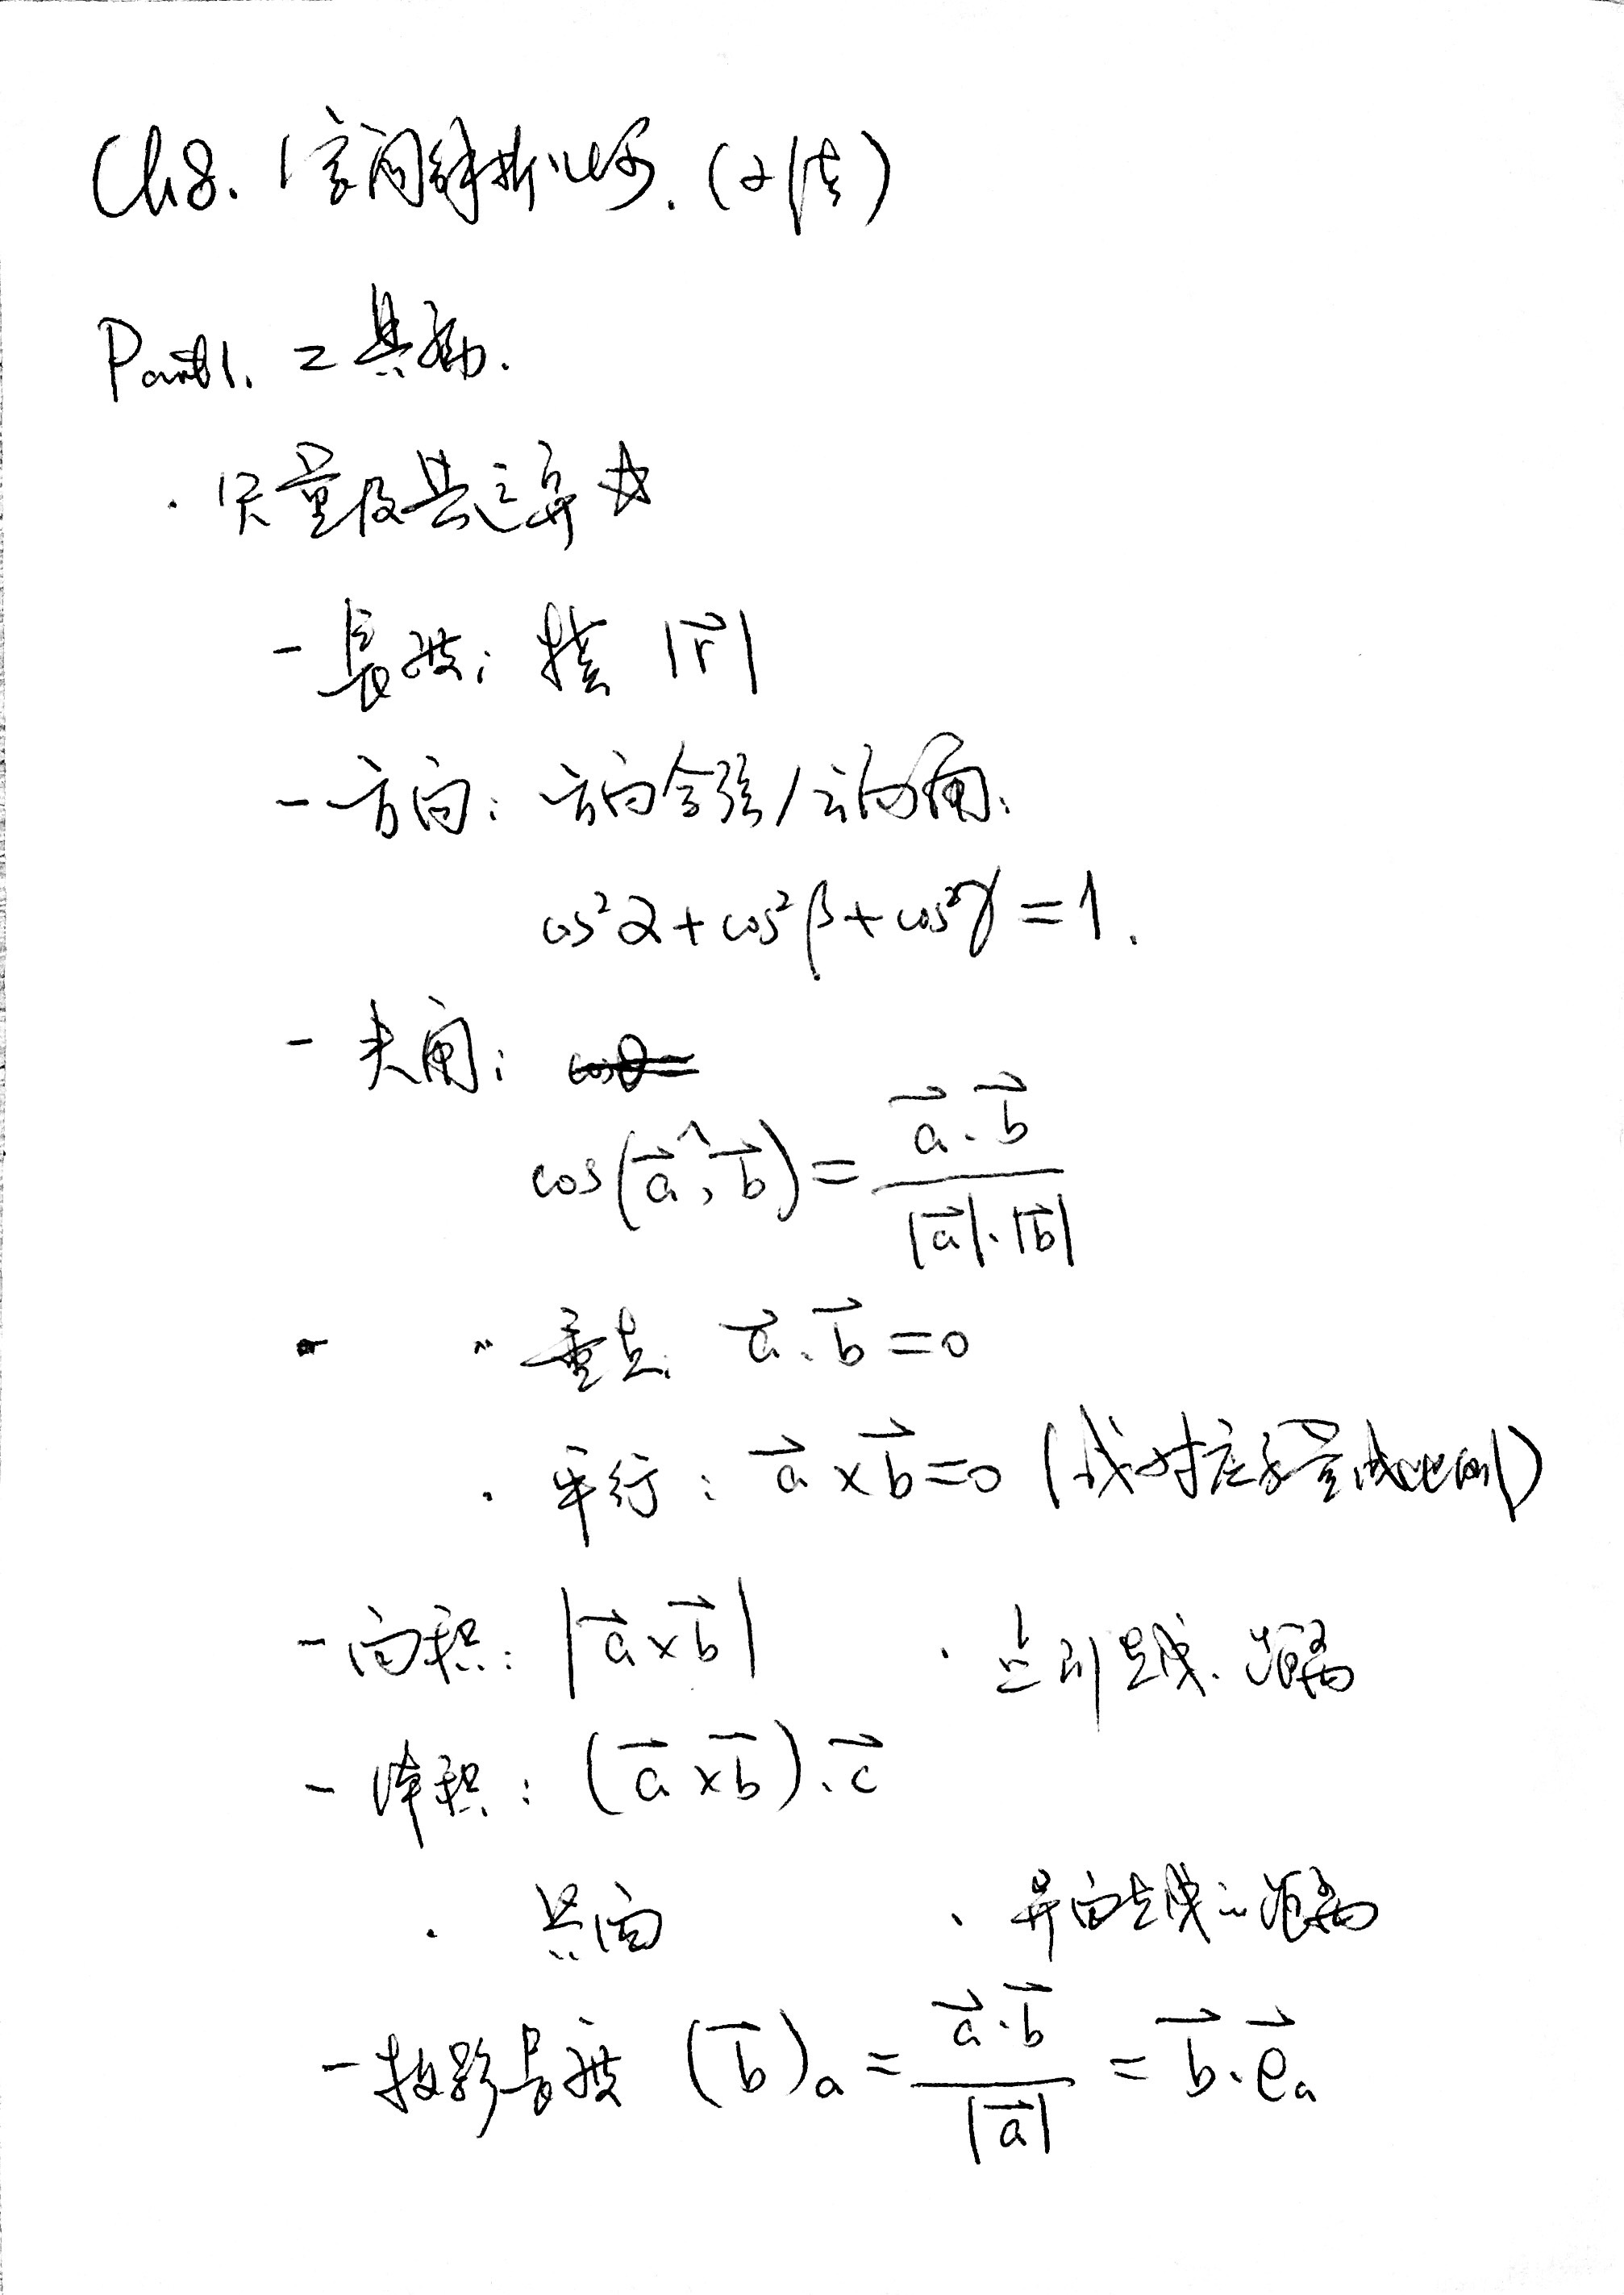
\includegraphics{./images/ch8/review/1.jpg}}\quad\quad\quad
\resizebox{!}{8cm}{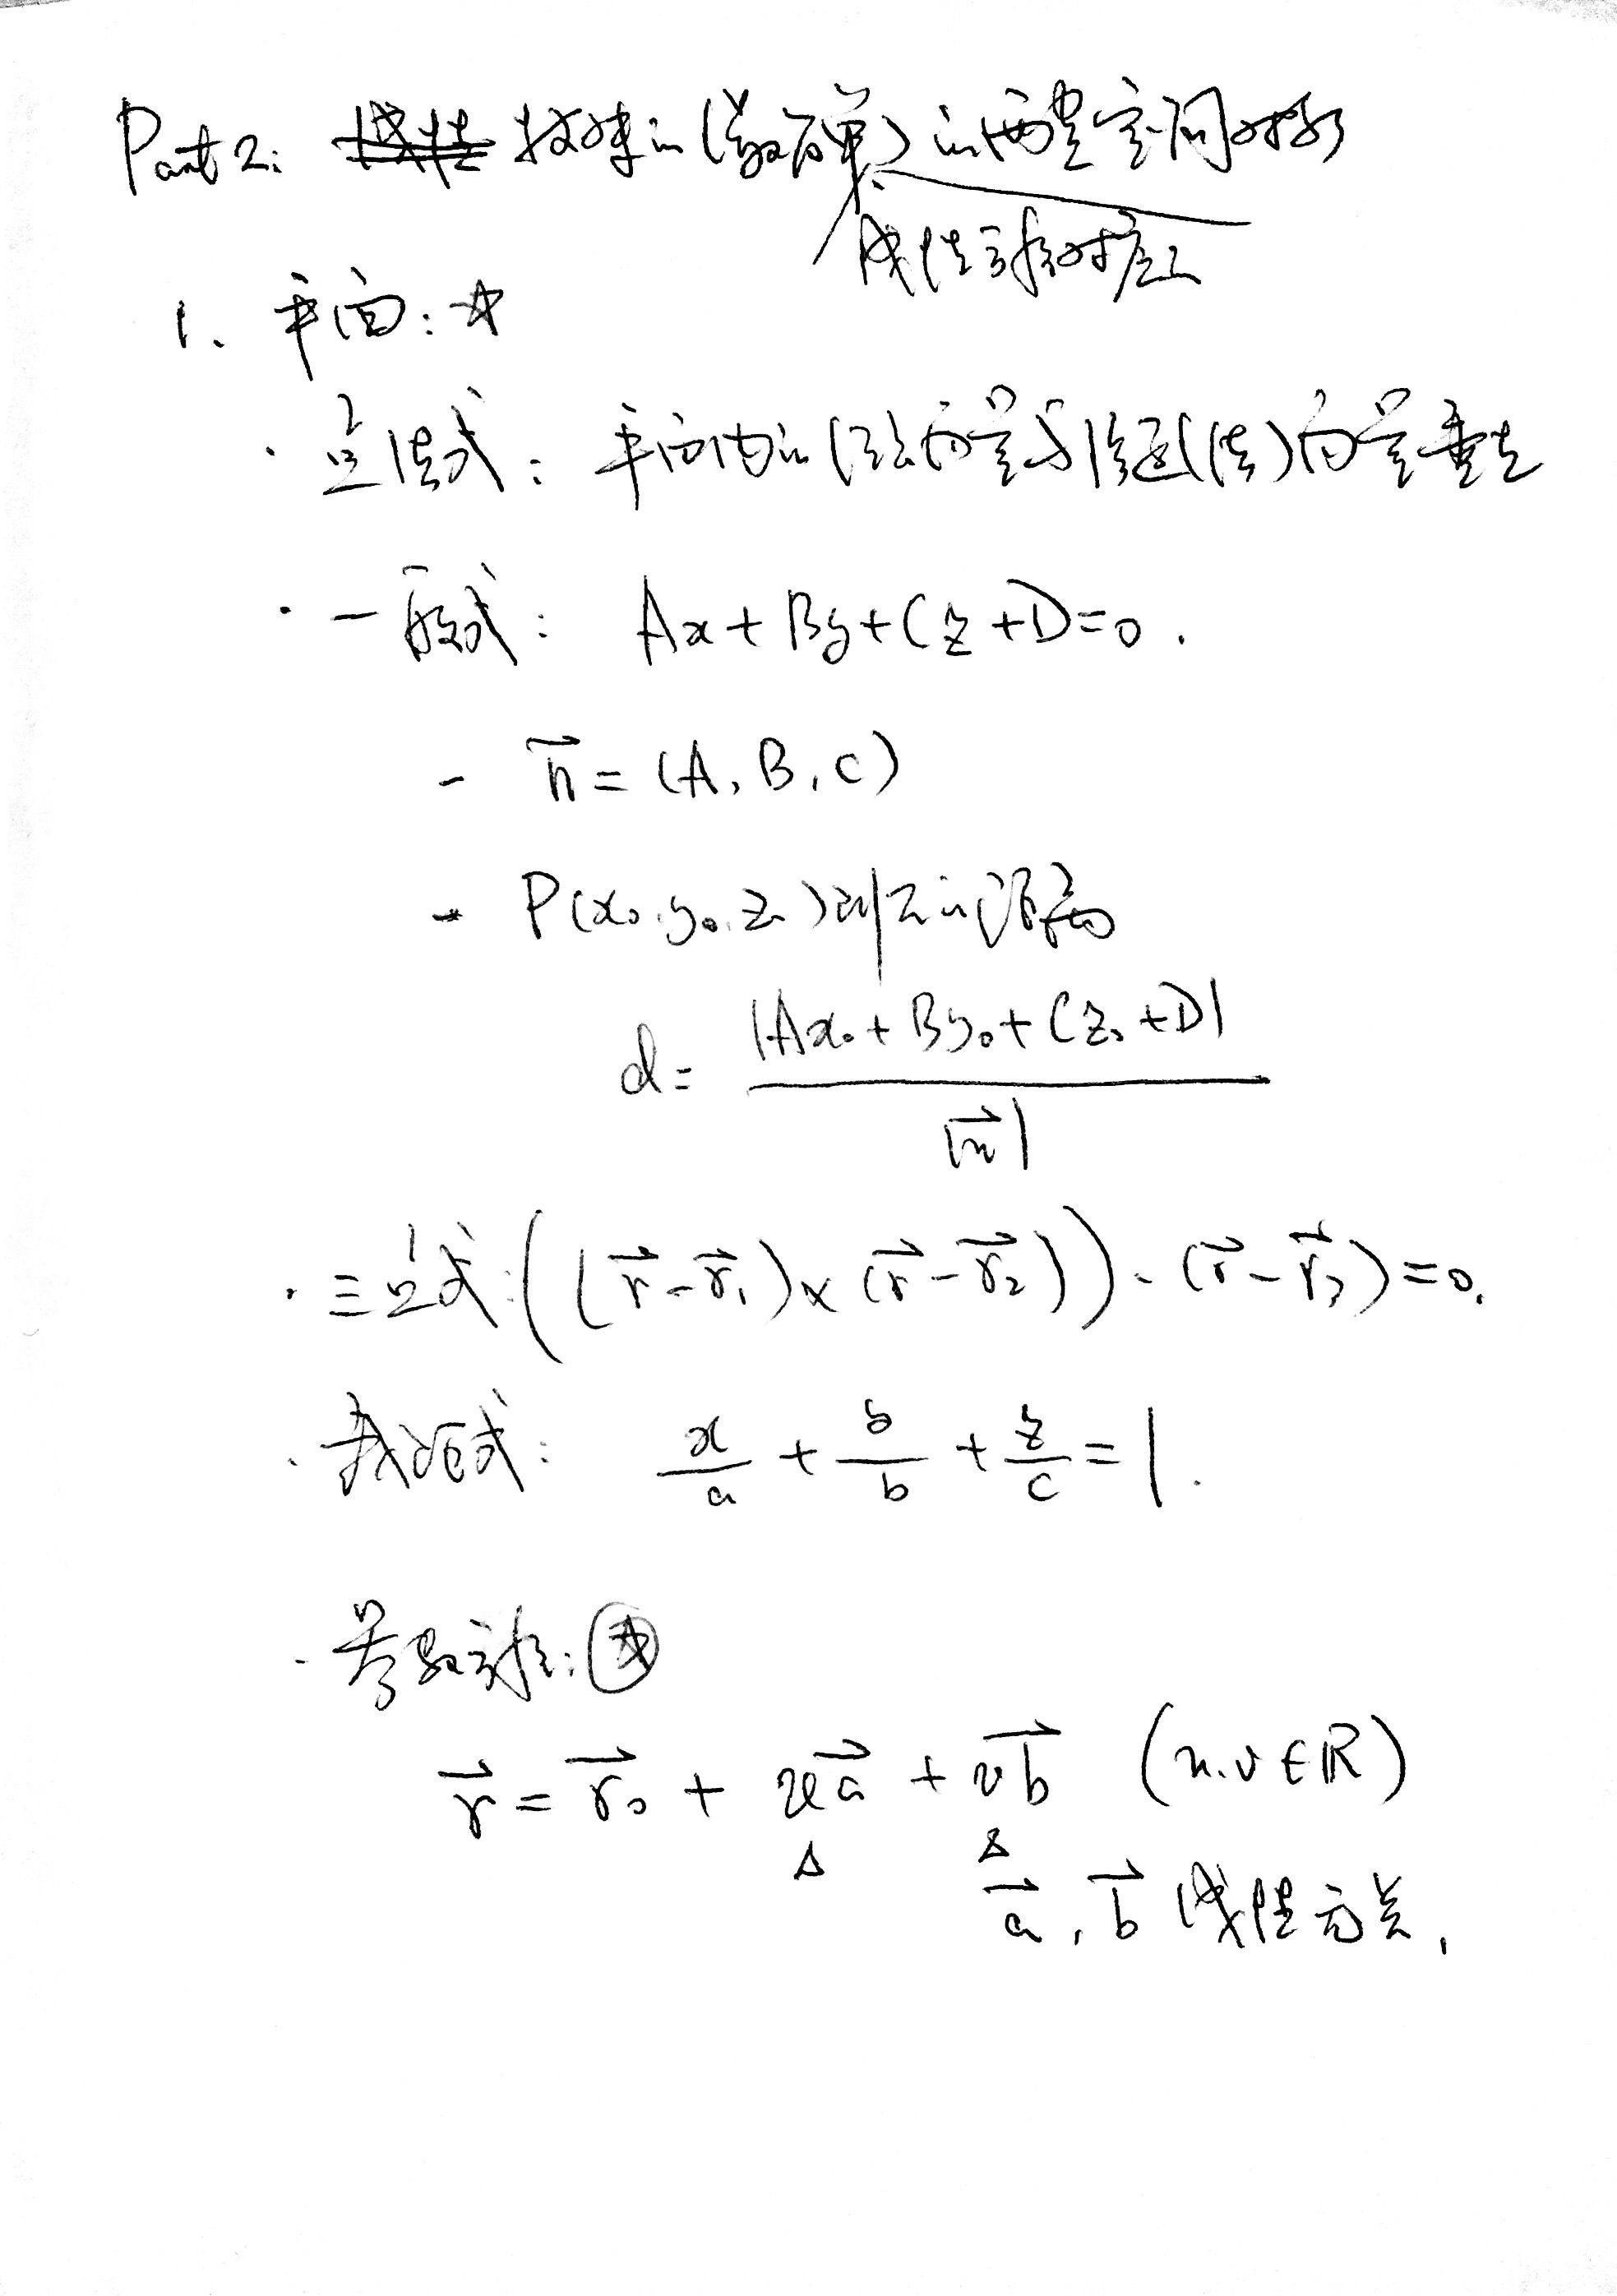
\includegraphics{./images/ch8/review/2.jpg}}

\resizebox{!}{8cm}{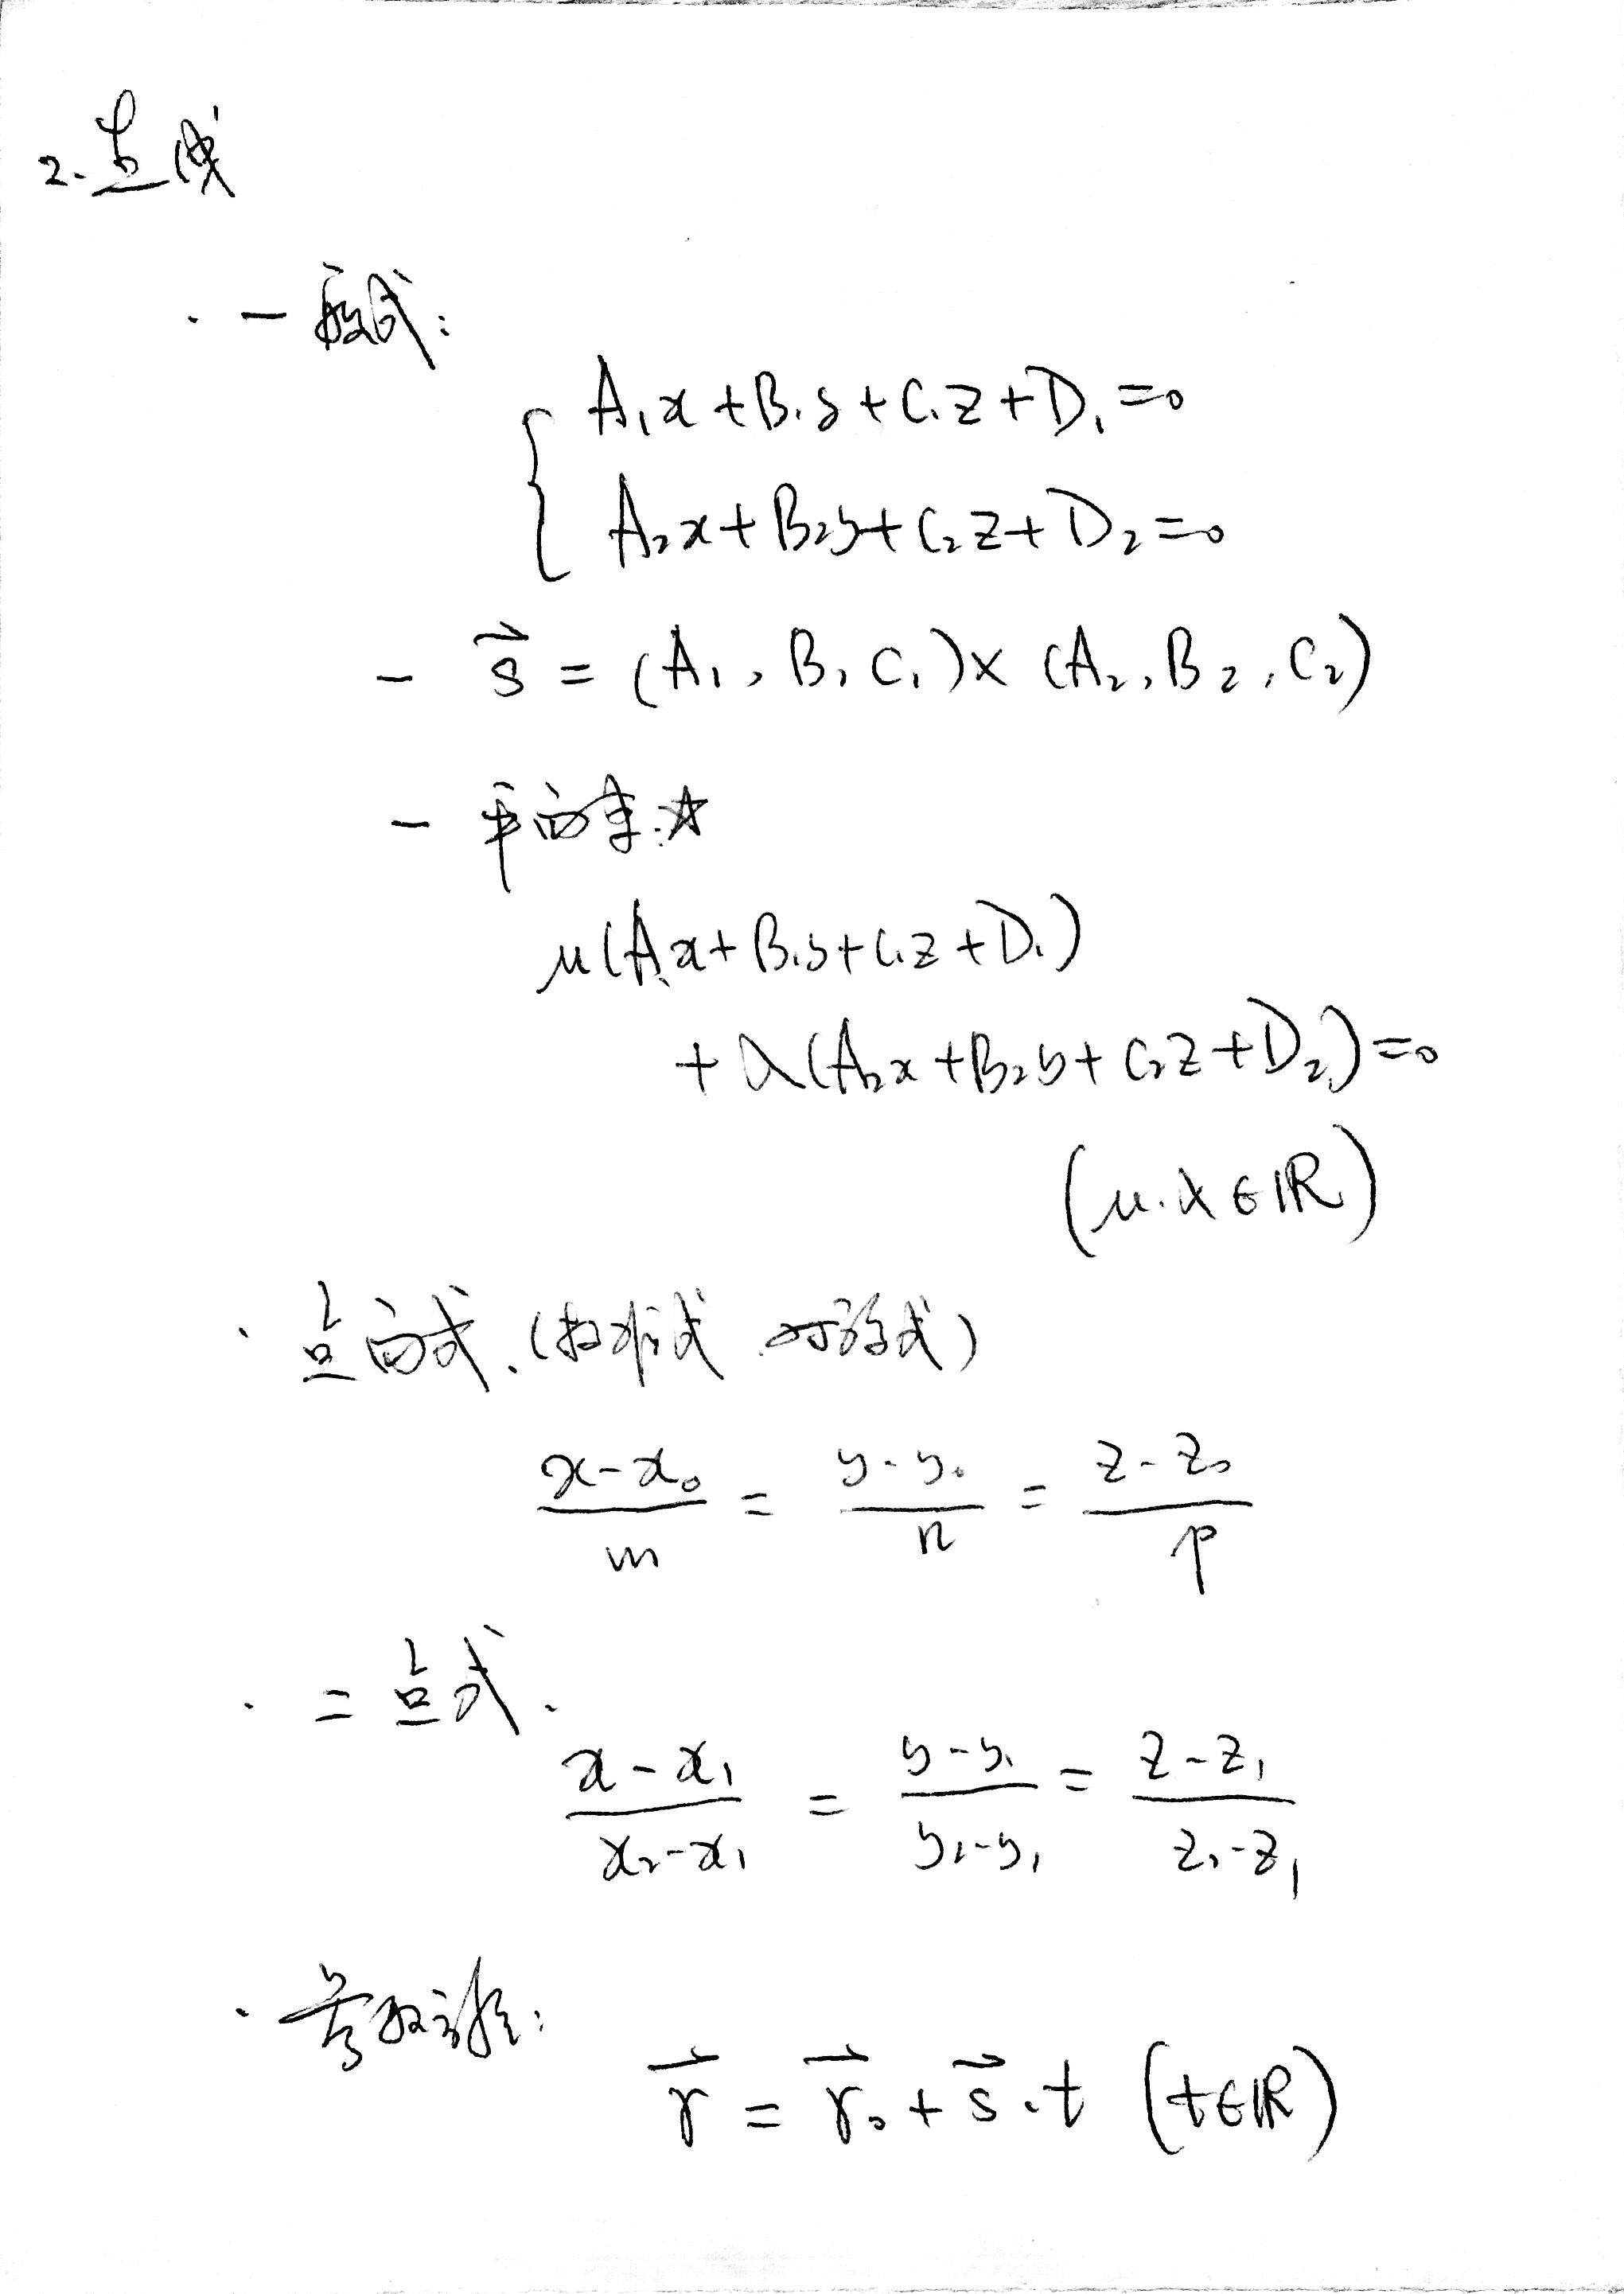
\includegraphics{./images/ch8/review/3.jpg}}\quad\quad\quad
\resizebox{!}{8cm}{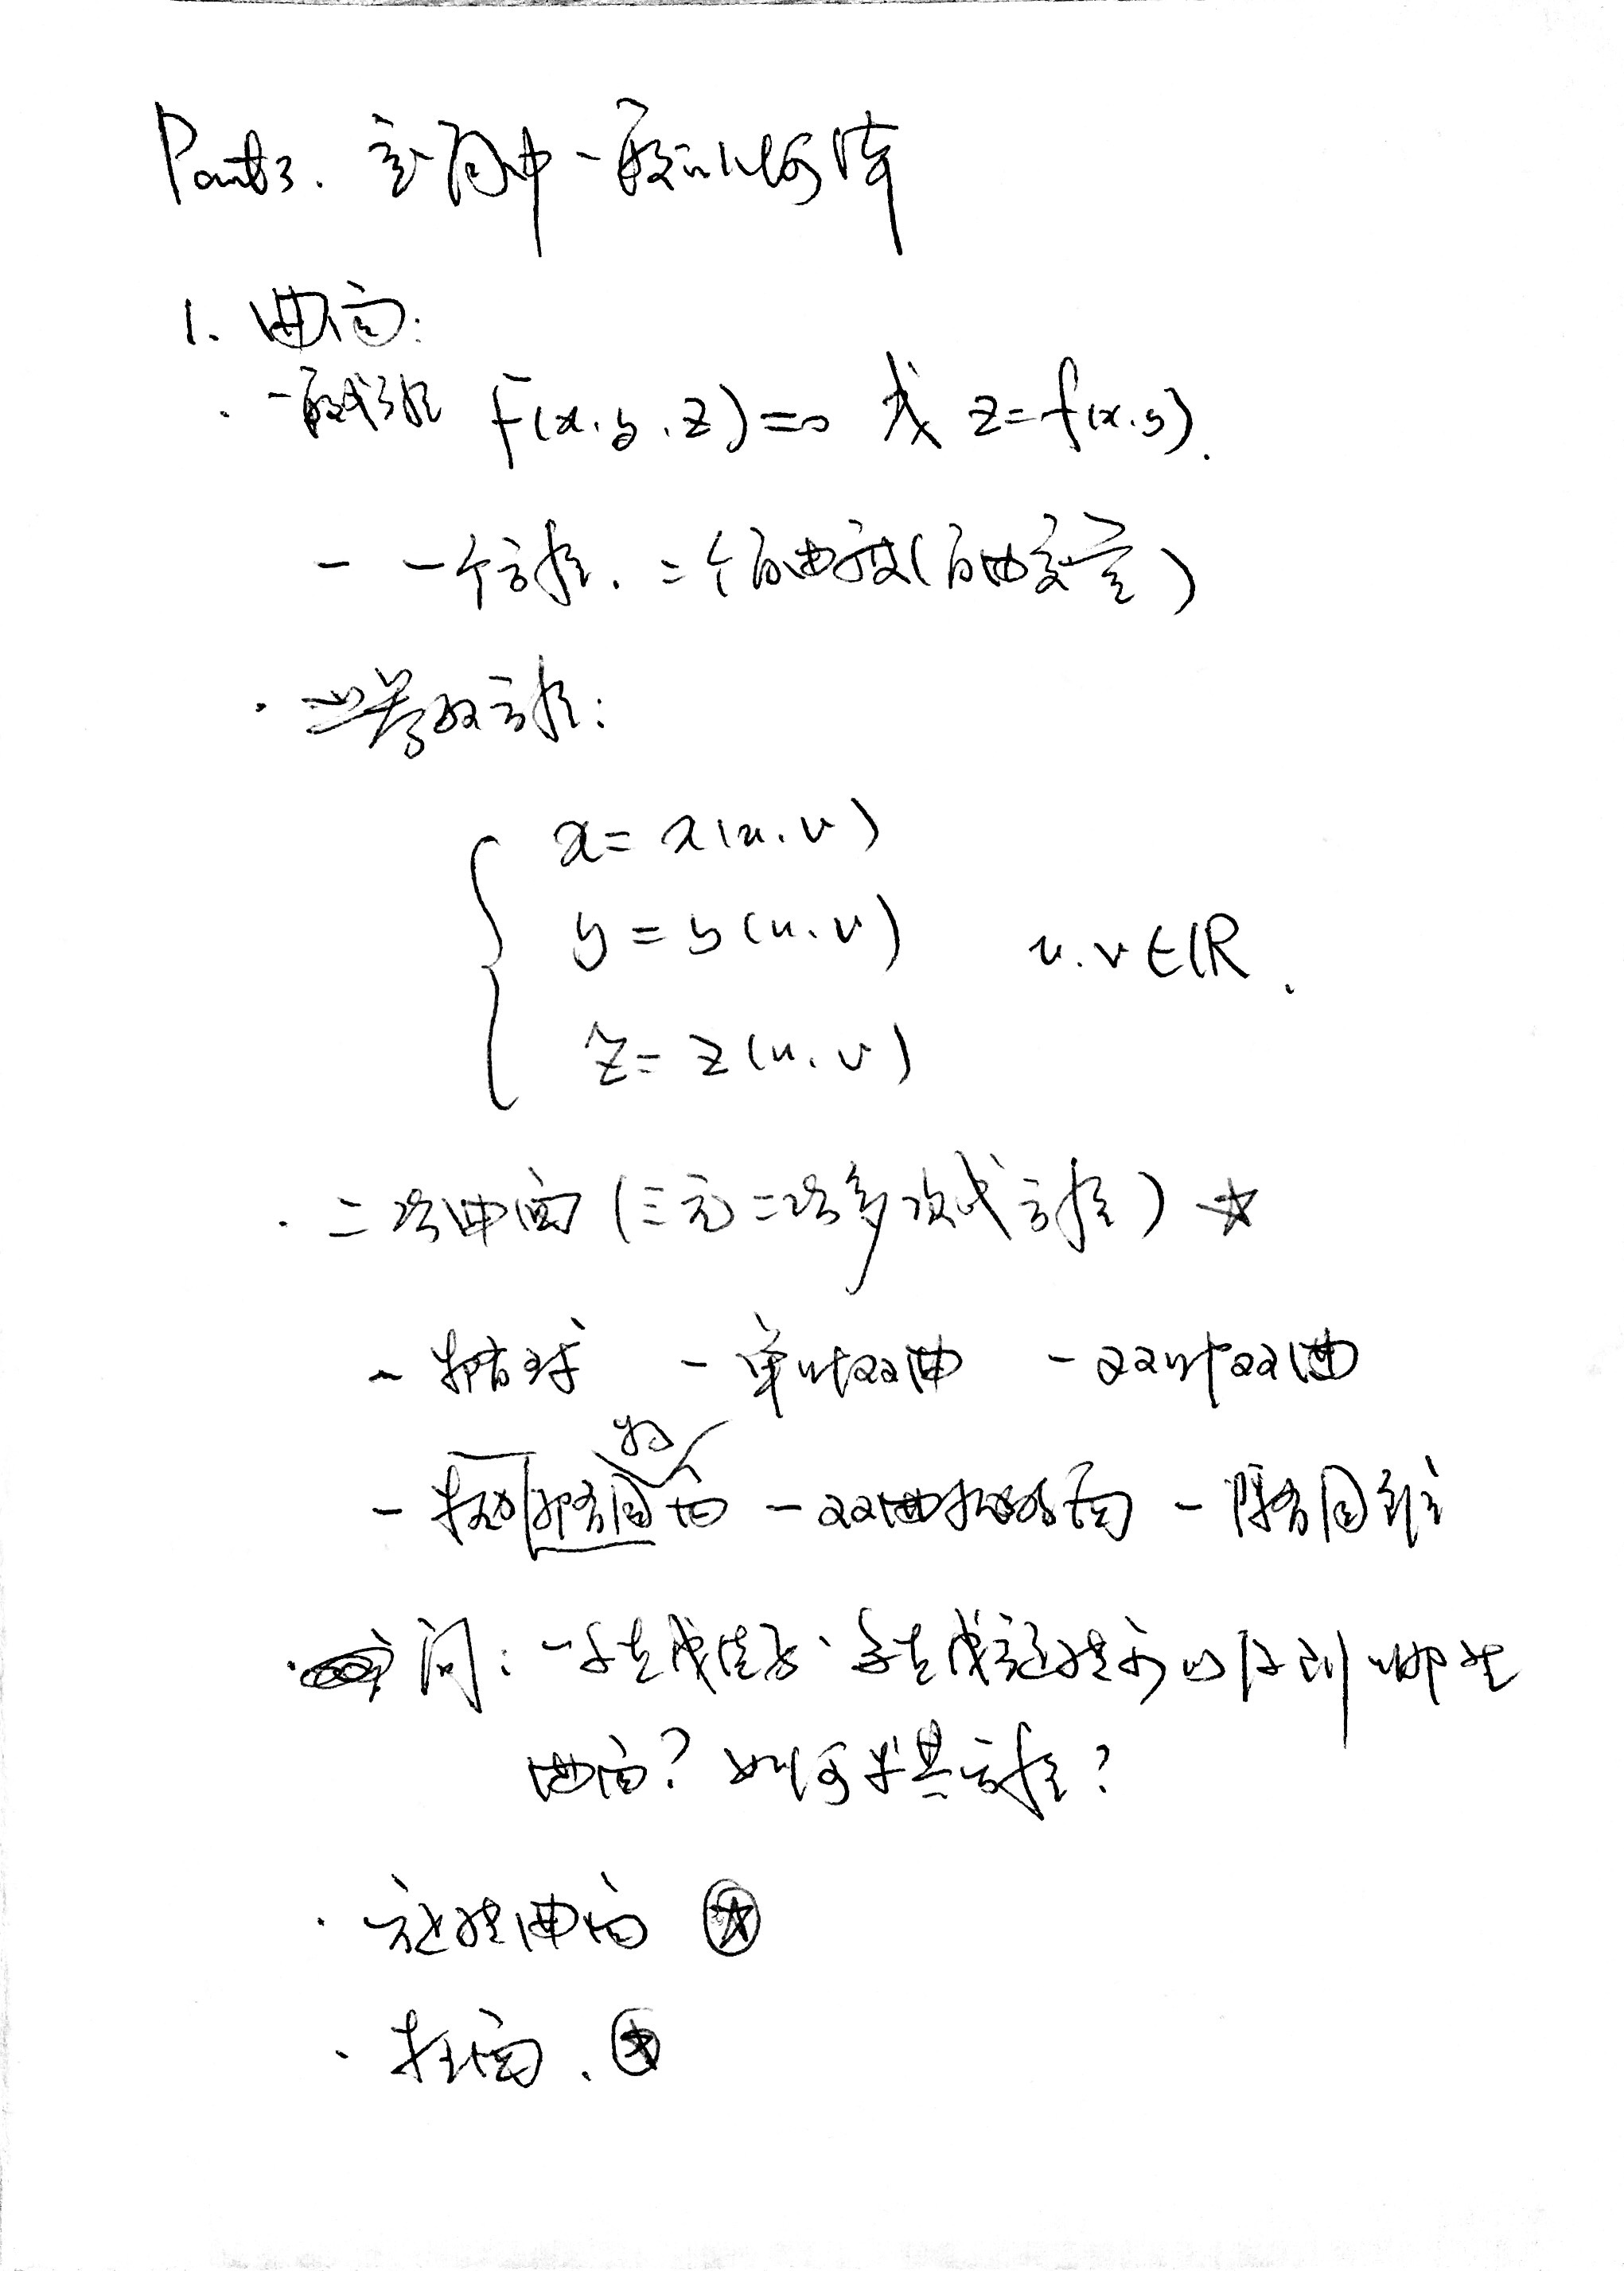
\includegraphics{./images/ch8/review/4.jpg}}

\resizebox{!}{8cm}{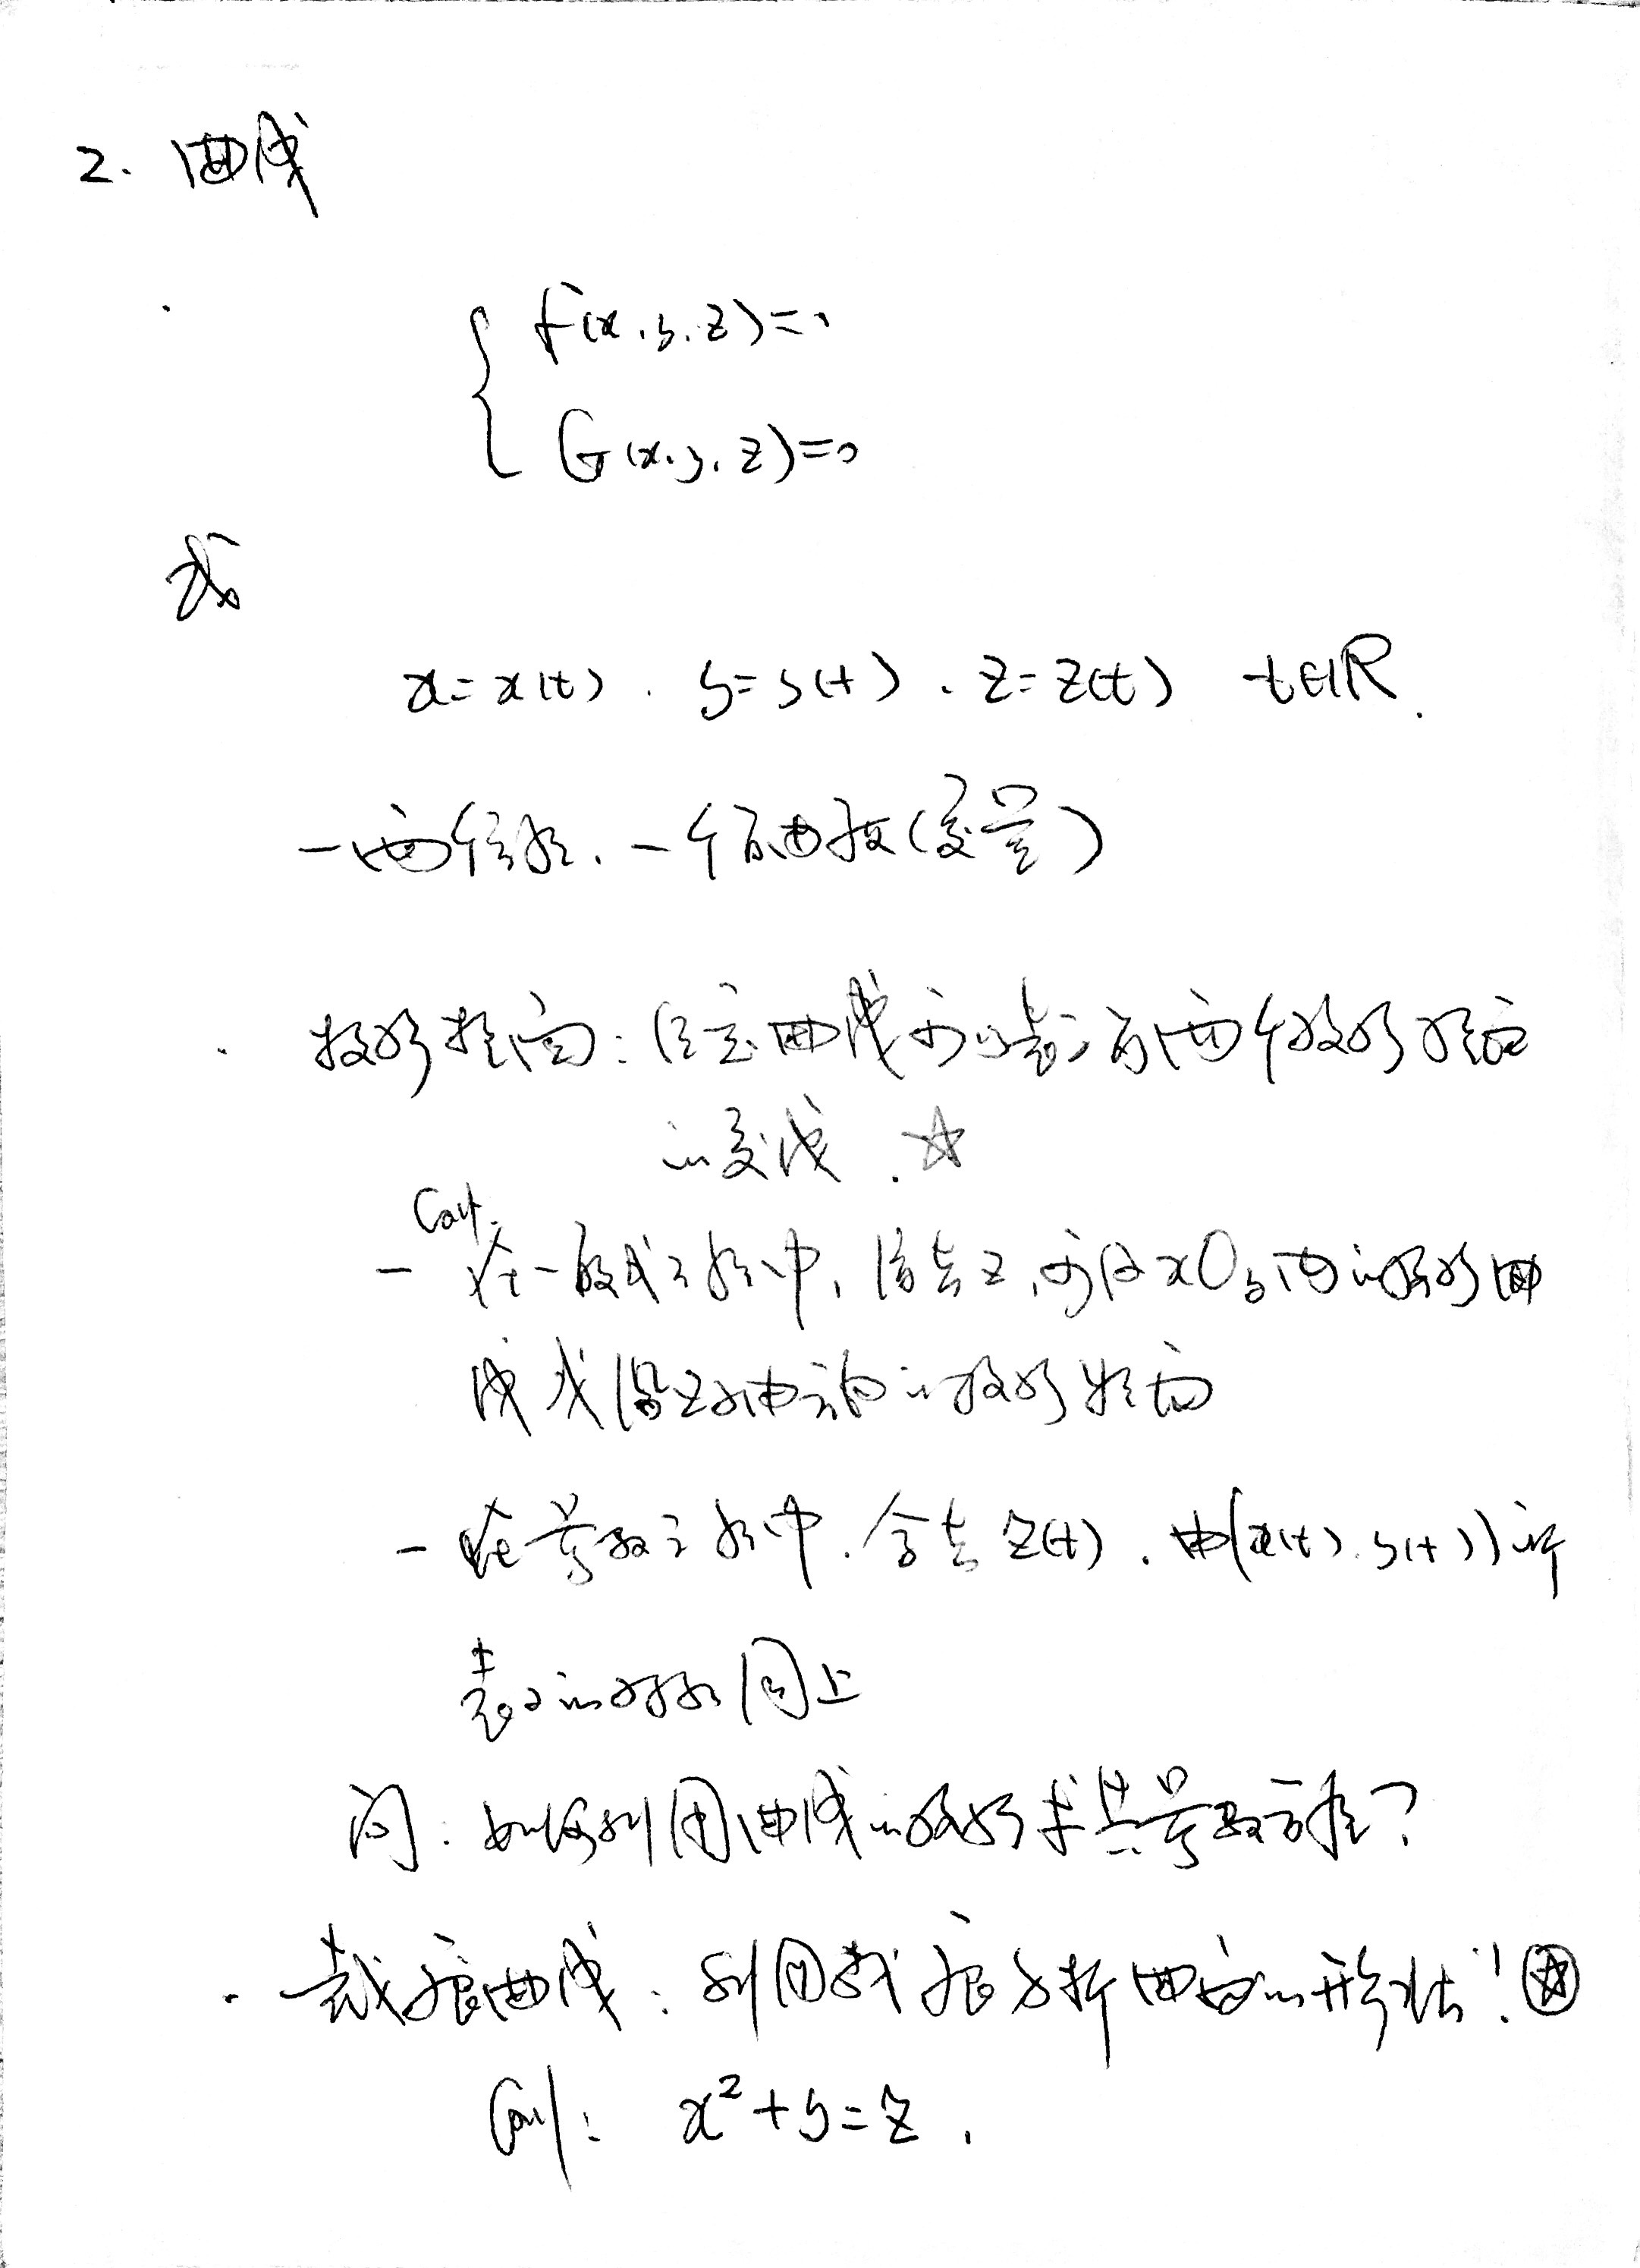
\includegraphics{./images/ch8/review/5.jpg}}

\fi